%%%%%%%%%%%%%%%%%%%%%%%%%%%%%%%%%%%%%%%%%%%%%%%%%%%%
% Document type, global settings, and packages
%%%%%%%%%%%%%%%%%%%%%%%%%%%%%%%%%%%%%%%%%%%%%%%%%%%%

\documentclass[english,11pt,twoside]{report}   %12 point font for Times New Roman
\usepackage[a4paper,hmargin=3.5cm,vmargin=5.3cm,head=1.5cm,foot=3.2cm]{geometry}
\usepackage[bookmarks=true, hidelinks]{hyperref}     % hyperlink
\usepackage{url} 
\usepackage[acronym]{glossaries}
\usepackage[bibencoding=utf8,backend=biber,style=numeric,sorting=none,bibstyle=phys]{biblatex} 
\addbibresource{references.bib}  
\makeglossaries

% https://tex.stackexchange.com/questions/47576/combining-ifxetex-and-ifluatex-with-the-logical-or-operation
\usepackage{ifxetex,ifluatex}

\newif\ifxetexorluatex
\ifxetex
  \xetexorluatextrue
\else
  \ifluatex
    \xetexorluatextrue
  \else
    \xetexorluatexfalse
  \fi
\fi

\ifxetexorluatex
  % To fix LaTeX command is already defined error, load amssymb before unicode-math
  % https://tex.stackexchange.com/a/547153/56364
  % \usepackage{stix}
  \usepackage{amssymb}
  \usepackage{fontspec}
  \usepackage{unicode-math}

  \defaultfontfeatures{Scale=MatchLowercase,Ligatures=TeX}
  % \setmainfont{STIX Two Text}
  \setmainfont{Noto Serif}
  \setmathfont{TeX Gyre Schola Math}
  \usepackage[scale=0.8]{noto-mono}
  \setmonofont{Noto Sans Mono}
  % small url fonts
  \renewcommand{\UrlFont}{\ttfamily\small}

  \ifxetex
    % https://gist.github.com/dlimpid/5454229
    % Use xeCJK in XeLaTeX
    \usepackage{xeCJK}
    \xeCJKsetup{%
      CJKspace=true,% % true이면 띄어쓰기 사용. 중국어, 일어는 필요 없을수도
      % CJKmath=true,%  % true면 math environment 안에서 CJK 글자 사용
      CJKecglue={}%   % Western과 CJK 사이의 공백 지정: {}로 간격을 없앰
    }
    \setCJKmainfont[
      Path=fonts/,
      Extension=.otf,
      BoldFont=NotoSerifkr-Bold,
      AutoFakeSlant,
      Ligatures=TeX]{NotoSerifkr-Regular.otf}
    \setCJKsansfont[
      Path=fonts/,
      Extension=.otf,
      BoldFont=NotoSerikr-Bold,
      AutoFakeSlant,
      Ligatures=TeX]{NotoSerifkr-Regular.otf}
    \setCJKmonofont[
      Path=fonts/,
      Extension=.ttf,
      BoldFont=NotoSansMono-Bold,
      AutoFakeSlant,
      Ligatures=TeX]{NotoSansMono-Regular.ttf}
  \fi

  \ifluatex
    \usepackage[hangul]{luatexko}
    \setmainhangulfont[
      Path=fonts/,
      UprightFont=*-Regular,
      BoldFont=*-Bold,
      Extension=.otf,
      AutoFakeSlant,
      Ligatures=TeX]{NotoSerifkr}
    \hangulbyhangulfont=1
    \setmainfont{Noto Serif}
    \setmathfont{TeX Gyre Schola Math}
    \usepackage[scale=0.8]{noto-mono}
    \setmonofont{Noto Sans Mono}
  \fi
\else
  % pdflatex doesn't work due to siunitx and kotex conflict
  % https://t.co/PgBfFh9rTU?amp=1
  \usepackage{amsmath,amsthm,amsfonts}
  \usepackage[T1]{fontenc}
  \usepackage[utf8]{inputenc}
  \usepackage[finemath]{kotex} % Use kotex in PDFLaTeX
  % \usepackage{CJKutf8}
  \usepackage{textcomp} % provide euro and other symbols

  % use nanum font in Korean
  \usepackage{dhucs-nanumfont}
  % otherwise, use Noto fonts
  \usepackage{noto}
\fi

\ifxetex
  \XeTeXinputnormalization=1
\fi

\renewcommand{\floatpagefraction}{0.1} % one figure in one page

\usepackage[english]{babel}    % babel set language
\usepackage{csquotes}

\usepackage{setspace}   %use this package to set linespacing as desired
\doublespacing
\usepackage{afterpage}    % separate page for floats and tables
\usepackage{titlefoot}    % keywords on footnote
\usepackage{bookmark}
\usepackage[explicit]{titlesec}  %title control and formatting
\usepackage[titles]{tocloft}  %table of contents control and formatting
\usepackage[page]{appendix}  %for appendices
\usepackage[normalem]{ulem}  %for underlined section titles

\usepackage{graphicx}  %for images and plots
\usepackage[figuresright]{rotating}  %for rotated, landscape images
\usepackage{adjustbox}    % fit table to page width
\usepackage{algorithm}      % algorithm
\usepackage{algpseudocode}  % algorithm

\usepackage{booktabs}     % proessional-quality tables
\usepackage{multicol} 		% use multicol in table
\usepackage{multirow} 		% use multirow in table

\usepackage{xcolor}			  % color fonts
\usepackage[super]{nth}		% th
\usepackage{siunitx}		  % SI unit
\usepackage[noabbrev,nameinlink]{cleveref}		% for multiple cross-reference
\usepackage[intoc]{nomencl}  % nomenclature
\usepackage{graphicx}
\usepackage{subcaption}

\makenomenclature
\setlength{\nomitemsep}{-\parsep}
\setlength{\nomlabelwidth}{1.7cm}

%%%%%%%%%%%%%%%%%%%%%%%%%%%%%%%%%%%
% Bibliography
%%%%%%%%%%%%%%%%%%%%%%%%%%%%%%%%%%%

%Add your bibliography file here
\addbibresource{references.bib}

% escape % in abstract of bibfile (due to it is perl program)
\DeclareSourcemap{
  \maps[datatype = bibtex]{
    \map{
       \step[fieldsource = abstract,
          match = \regexp{([^\\])\%},
          replace = \regexp{$1\\\%}]
    }
  }
}

% prevent certain fields in references from printing in bibliography
\AtEveryBibitem{\clearfield{abstract}}
\AtEveryBibitem{\clearlist{abstract}}

\AtEveryBibitem{\clearfield{issn}}
\AtEveryBibitem{\clearlist{issn}}

\AtEveryBibitem{\clearfield{language}}
\AtEveryBibitem{\clearlist{language}}

\AtEveryBibitem{\clearfield{doi}}
\AtEveryBibitem{\clearlist{doi}}

\AtEveryBibitem{\clearfield{url}}
\AtEveryBibitem{\clearlist{url}}

\AtEveryBibitem{%
  \ifentrytype{online}
    {}
    {\clearfield{urlyear}\clearfield{urlmonth}\clearfield{urlday}}}

% footnote for keywords in abstract
% https://tex.stackexchange.com/questions/30720/footnote-without-a-marker
\newcommand\blfootnote[1]{%
  \begingroup
  \renewcommand\thefootnote{}\footnote{#1}%
  \addtocounter{footnote}{-1}%
  \endgroup
}
%%%%%%%%%%%%%%%%%%%%%%
% Start of Document
%%%%%%%%%%%%%%%%%%%%%%
\newacronym{cbrs}{CBRS}{Citizens Broadband Radio Service}
\newacronym{gan}{GAN}{Generative Adversarial Network}
\newacronym{dsa}{DSA}{Dynamic Spectrum Access}
\newacronym{vq-vae}{VQ-VAE}{Vector Quantized Variational Autoencoder}
\newacronym{cnn}{CNN}{Convolutional Neural Network}
\newacronym{fid}{FID}{Fréchet Inception Distance}
\newacronym{ddpm}{DDPM}{Denoising Diffusion Probabilistic Model}
\newacronym{pal}{PAL}{Priority Access License}
\newacronym{gaa}{GAA}{General Authorized Access}
\newacronym{fcc}{FCC}{Federal Communications Commission}
\newacronym{sas}{SAS}{Spectrum Access System}
\newacronym{jdl}{JDL}{Joint Distribution Learning}
\newacronym{edm}{EDM}{Elucidated Diffusion Models}
\newacronym{api}{API}{Application Programming Interface}
\newacronym{usrp}{USRP}{Universal Software Radio Peripheral}
\newacronym{cbsd}{CBSD}{Citizens Broadband Radio Service Device}
\newacronym{cbam}{CBAM}{Convolutional Block Attention Module}
\newacronym{gap}{GAP}{Global Average Pooling}
\newacronym{fc}{FC}{Fully Connected}
\newacronym{pca}{PCA}{Principal Component Analysis}
\newacronym{tvws}{TVWS}{TV White Spaces}
\newacronym{sibi}{SIBI}{System Information Block}
\newacronym{mnc}{MNC}{Mobile Network Code}
\newacronym{itu}{ITU}{International Telecommunication Union}
\newacronym{lsa}{LSA}{Licensed Shared Access} 
\begin{document}

%%%%%%%%%%%%%%%%%%%%%%%%%%%%%%%%%%%%%
% Cover Page
%%%%%%%%%%%%%%%%%%%%%%%%%%%%%%%%%%%%%

%% Define your thesis title, your name, your school, and your month and year of graduation here
\newgeometry{top=7.13cm,bottom=4.75cm,right=4.17cm,left=4.17cm}
\newcommand{\coverTitle}{Dynamic Spectrum Sharing Using Deep Learning and Generative Artificial Intelligence Models}
\newcommand{\coverName}{Amanda Sheron Gamage}

%%%%%%%%%%%%%%%%%%%%%%%%%%%%%%%%%%%%%%%%%%%%%%%%%%%%%%%%%
% Do not edit these lines unless you wish to customize
% the template
%%%%%%%%%%%%%%%%%%%%%%%%%%%%%%%%%%%%%%%%%%%%%%%%%%%%%%%%%

\begin{titlepage}
\clearpage\thispagestyle{empty}
\begin{center}

{\fontsize{18pt}{20pt} \selectfont \coverTitle \vspace{3.5cm} \par}

{\fontsize{18pt}{20pt} \selectfont \coverName \vspace{3.5cm} \par}
{\fontsize{18pt}{20pt} \selectfont
School of Electrical and Electronic Engineering \par
The Graduate School  \par
Yonsei University \par}
\vfill

\end{center}
\end{titlepage}



\currentpdfbookmark{Cover Page}{coverPage}  %add PDF bookmark for this page

%%%%%%%%%%%%%%%%%%%%%%%%%%%%%%%%%%%%%
% Title Page
%%%%%%%%%%%%%%%%%%%%%%%%%%%%%%%%%%%%%

% define title page margin
% \newgeometry{top=1in,bottom=1in,right=0.5in,left=1.5in}
%% Define your thesis title, your name, your school, and your month and year of graduation here
\newgeometry{top=4.75cm,bottom=3.56cm,right=4.17cm,left=4.17cm}

\newcommand{\thesisTitle}{Dynamic Spectrum Sharing Using Deep Learning and Generative Artificial Intelligence Models}
\newcommand{\mythesisTitle}{Dynamic Spectrum Sharing Using Deep Learning and Generative Artificial Intelligence Models}
\newcommand{\yourName}{Amanda Sheron Gamage}
\newcommand{\yourMonth}{June}
\newcommand{\yourYear}{2025}

%%%%%%%%%%%%%%%%%%%%%%%%%%%%%%%%%%%%%%%%%%%%%%%%%%%%%%%%%
% Do not edit these lines unless you wish to customize
% the template
%%%%%%%%%%%%%%%%%%%%%%%%%%%%%%%%%%%%%%%%%%%%%%%%%%%%%%%%%

\begin{titlepage}
\clearpage\thispagestyle{empty}
\begin{center}

{\fontsize{16pt}{20pt} \selectfont \mythesisTitle \vspace{2.40cm} \par}
\vspace{0.90cm}
{\fontsize{16pt}{20pt} \selectfont Advisor Prof. Seong-Lyun Kim \vspace{2.56cm} \par}
{\fontsize{16pt}{15pt}
\selectfont
    A Dissertation Submitted to the \par
    School of Electrical and Electronic Engineering \par
    and the Committee on Graduate School \par
    of Yonsei University in partial fulfillment of the \par
    requirements for the degree of \par
    Master of Science \\
    \vspace{2.56cm} 
    \par}

\begin{doublespacing}
    {\fontsize{16pt}{18pt}
    \selectfont 
    \vspace{0.95cm}
    \yourName \par
    \vspace{0.95cm}
    \yourMonth{} \yourYear{} \par
}
\vfill
\par

\end{doublespacing}
\end{center}
\end{titlepage}



\currentpdfbookmark{Title Page}{titlePage}  %add PDF bookmark for this page

%%%%%%%%%%%%%%%%%%%%%%%%%%%%%%%%%%%%%
% Approval Page
%%%%%%%%%%%%%%%%%%%%%%%%%%%%%%%%%%%%%

\newgeometry{top=4.15cm,bottom=4.15cm,right=4.17cm,left=4.17cm}
%% Define your committee members. If you have less than 6, simple delete/comment the unused lines
\newcommand{\approvalAuthor}{Gamage Amanda Sheron }
\newcommand{\committeeMemberOne}{Thesis Supervisor: Prof. Seong Lyun Kim}
\newcommand{\committeeMemberTwo}{Prof.  Jeonghun Park }
\newcommand{\committeeMemberThree}{Prof. Jemin Lee}


%%%%%%%%%%%%%%%%%%%%%%%%%%%%%%%%%%%%%%%%%%%%%%%%%%%%%%%%%
% Do not edit these lines unless you wish to customize
% the template
% Remove committeeMemberFour and committeeMembmerFive 
% if you are master student
%%%%%%%%%%%%%%%%%%%%%%%%%%%%%%%%%%%%%%%%%%%%%%%%%%%%%%%%%

\begin{titlepage}
\clearpage\thispagestyle{empty}

\begin{singlespacing}

\centering

\large{
	This certifies that the dissertation of \approvalAuthor  is approved.
}

\vspace{2.97cm}		%adjust the number in front of "\baselineskip" for alignment

\par\rule{6.5cm}{0.8pt}\null \\
\large{\committeeMemberOne} \\
\vspace{1.78cm}

\par\rule{6.5cm}{0.8pt}\null \\
\large{\committeeMemberTwo} \\
\vspace{1.78cm}

\par\rule{6.5cm}{0.8pt}\null \\
\large{\committeeMemberThree} \\
\vspace{1.78cm}



{\fontsize{14pt}{24pt}
	\selectfont
	Graduate School \par
	Yonsei University \par
	June 2025 \par
}
\vfill
\end{singlespacing}
\end{titlepage}


%%%%%%%%%%%%%%%%%%%%%%%%%%%%%%%%%%%%%
% Acknowledgments
%%%%%%%%%%%%%%%%%%%%%%%%%%%%%%%%%%%%%

% \pagenumbering{roman}
% \addcontentsline{toc}{chapter}{Acknowledgments}
% \setcounter{page}{5} % set the page number appropriately based on the number of intro pages
\clearpage
\newgeometry{hmargin=3.5cm,vmargin=5.3cm,head=3.5cm,foot=3.2cm}
\begin{centering}
\textbf{ACKNOWLEDGEMENTS}\\
\vspace{\baselineskip}
\end{centering}

As I complete my master’s degree, I am grateful to have been surrounded by wonderful people, which allowed me to enjoy a happy graduate school life. 
I would like to express my heartfelt thanks to the precious individuals who helped me finish this journey well.

First, I extend my deep gratitude to my advisor, Professor Seong Lyun Kim, for his invaluable guidance and support throughout my research. 
His expertise and encouragement have been instrumental in shaping my academic journey. 
I am also thankful to my committee members, Professor Jeonghun Park and Professor Jemin Lee, for their insightful feedback and support.

I would like to express my appreciation to all the members of the RAMO laboratory for their support and friendship. I am especially grateful to
 혜린 for assisting me with my research and for helping me navigate the nuances of living in Korea. I would also like to thank 민규, 수진, 최진혁, 
 김진혁, and 혜성 for their help during various stages of my research. My thanks extend to all RAMO members, including 여선, 박지, 명진, 중호, 이지, 윤서, 
 Changjie, Dr. 오승은, and Dr. Arman Ahmadian, for their invaluable assistance and companionship throughout my time in the lab. Their camaraderie 
 made my experience not only productive but truly enjoyable. I will forever cherish the memories I made with the incredible people I met through RAMO.

Next, I would like to express my gratitude to the Government of the Republic of Korea and the Ministry of Education for giving me the opportunity to 
pursue my studies in Korea through the Global Korea Scholarship (GKS) program.

Finally, I would like to express my deepest gratitude to my parents, grandmother, sister, Tharindu, and friends. Though they were far away, their 
unwavering support, love, and belief in me have been a constant source of strength. I am truly thankful for their presence in my life.

\pagenumbering{gobble}
\thispagestyle{empty}
\clearpage


%\addtocontents{toc}{\cftpagenumbersoff{chapter}}

%\currentpdfbookmark{Acknowledgments}{acknowledgments}
%\addtocontents{toc}{\cftpagenumberson{chapter}}
% Set location of page numbering as just below text body
\newgeometry{hmargin=3.5cm,vmargin=5.3cm,head=1.5cm,foot=3.2cm,footskip=1cm}
%%%%%%%%%%%%%%%%%%%%%%%%%%%%%%%%%%%%%
% Table of Contents
%%%%%%%%%%%%%%%%%%%%%%%%%%%%%%%%%%%%%
\pagenumbering{roman}
\setcounter{page}{1} % set the page number appropriately based on the number of intro pages
% Format for Table of Contents
\renewcommand{\cftchapdotsep}{\cftdotsep}  %add dot separators
\renewcommand{\cftchapfont}{\bfseries}  %set title font weight
\renewcommand{\cftchappagefont}{}  %set page number font weight
\renewcommand{\cftchappresnum}{Chapter }
\renewcommand{\cftchapaftersnum}{:}
\renewcommand{\cftchapnumwidth}{7em}
\renewcommand{\cftchapafterpnum}{\vskip\baselineskip} %set correct spacing for entries in single space environment
\renewcommand{\cftsecafterpnum}{\vskip\baselineskip}  %set correct spacing for entries in single space environment
\renewcommand{\cftsubsecafterpnum}{\vskip\baselineskip} %set correct spacing for entries in single space environment
\renewcommand{\cftsubsubsecafterpnum}{\vskip\baselineskip} %set correct spacing for entries in single space environment

%format title font size and position (this also applys to list of figures and list of tables)
\titleformat{\chapter}[display]
{\normalfont\bfseries\filcenter}{\chaptertitlename\ \thechapter}{0pt}{\MakeUppercase{#1}}

\renewcommand\contentsname{Table of Contents}

\begin{singlespace}
\tableofcontents
\end{singlespace}

\currentpdfbookmark{Table of Contents}{TOC}

\clearpage

%%%%%%%%%%%%%%%%%%%%%%%%%%%%%%%%%%%%%
% List of figures and tables
%%%%%%%%%%%%%%%%%%%%%%%%%%%%%%%%%%%%%

\addcontentsline{toc}{chapter}{List of Tables}
\begin{singlespace}
	\setlength\cftbeforetabskip{\baselineskip}  %manually set spacing between entries
	\listoftables
\end{singlespace}

\clearpage

\addcontentsline{toc}{chapter}{List of Figures}
\begin{singlespace}
\setlength\cftbeforefigskip{\baselineskip}  %manually set spacing between entries
\listoffigures
\end{singlespace}

\clearpage

\printnomenclature
\clearpage

%%%%%%%%%%%%%%%%%%%%%%%%%%%%%%%%%%%%%%%%%%%%%%%%%%%%%%%%%%%%%%%%%
% This is the Abstract
%%%%%%%%%%%%%%%%%%%%%%%%%%%%%%%%%%%%%%%%%%%%%%%%%%%%%%%%%%%%%%%%%
\addcontentsline{toc}{chapter}{Abstract}
% \setcounter{page}{5} % set the page number appropriately based on the number of intro pages
\clearpage
\begin{centering}
\textbf{ABSTRACT}\\
\vspace{\baselineskip}
\end{centering}

\begin{flushright}
     Amanda Sheron Gamage \\
    School of Electrical and Electronic Engineering \\
    The Graduate School, Yonsei University
\end{flushright}

Dynamic spectrum sharing is a critical component in the efficient utilization of wireless communication resources, particularly within the Citizens Broadband Radio Service (CBRS) band. This thesis presents a novel end-to-end AI-driven framework for intelligent spectrum access that integrates generative modeling, supervised classification, and deep reinforcement learning (DRL). The system is designed to operate as a learning-based alternative to traditional Spectrum Access Systems (SAS), 
capable of real-time spectrum occupancy detection and autonomous channel decision-making.

To address the challenge of limited labeled data for training, we employ three types of generative AI models—Generative Adversarial Networks (GAN), 
Vector Quantized Variational Autoencoders (VQ-VAE), and Denoising Diffusion Probabilistic Models (DDPM)—to synthesize high-fidelity spectrogram images 
representing various CBRS scenarios, including interference and collision cases. These synthetic spectrograms are used to train a convolutional neural network (CNN) 
for binary classification of collision events. Experimental evaluations demonstrate that DDPM displays the best performance in terms of both visual fidelity 
and classification accuracy, significantly outperforming GAN and VQ-VAE.

A MATLAB-based CBRS simulation environment is developed, where a DRL agent, trained using a Deep Q-Network (DQN), interacts with the spectrum environment. 
The agent receives channel occupancy predictions from the CNN and learns to avoid collisions with Incumbent and Priority Access License (PAL) users while
 maximizing throughput on General Authorized Access (GAA) channels. Quantitative results show that the DQN agent trained with DDPM-generated data achieved 
 a mean reward of 79.65 with zero collisions per episode, indicating safe and effective channel selection. In comparison, the GAN-trained agent achieved a 
 higher reward of 86.78 but with a small number of collisions (0.74 per episode), while the VQ-VAE and original dataset agents suffered from higher collision 
 rates (12.6 and 17.44 per episode, respectively), despite lower or comparable rewards. These findings highlight the role of generative model quality in ensuring 
 both high performance and operational safety in spectrum access.

The thesis concludes that the integration of generative AI, deep classification, and DRL offers a scalable and intelligent solution to spectrum sharing in CBRS. 
The modular architecture, high-performance learning models, and simulation results provide a foundation for future extensions, including multi-channel scaling, 
real-time deployment, and unsupervised learning approaches for spectrum management.


\blfootnote{Keywords: Citizens Broadband Radio Service (CBRS), Generative Adversarial Networks (GAN), Vector Quantized Variational Autoencoders (VQ-VAE), 
Denoising Diffusion Probabilistic Models (DDPM), Deep Q-Network (DQN), Spectrum Access System (SAS), Dynamic Spectrum Sharing, Reinforcement Learning, 
Convolutional Neural Network (CNN).}
%\pagenumbering{gobble}  %remove page number on summary page




%%%%%%%%%%%%%%%%%%%%%%%%%%%%
%
% Chapters
%
%%%%%%%%%%%%%%%%%%%%%%%%%%%%

%%%%%%%%%%%%%%%%%%%%%%
% formatting
%%%%%%%%%%%%%%%%%%%%%%

% resume page numbering for rest of document
\clearpage
\pagenumbering{arabic}
\setcounter{page}{1} % set the page number appropriately

% Adjust chapter title formatting
\newcommand{\chapternamefont}{\scshape\Large}% Chapter name font
\newcommand{\chaptertitlefont}{\LARGE\bfseries}% Chapter title font
\titleformat{\chapter}[display]
{\normalfont\bfseries\chapternamefont\raggedright}{\MakeUppercase\chaptertitlefont\chaptertitlename\ \thechapter}{0pt}{\MakeUppercase{#1}}  %spacing between titles
\titlespacing*{\chapter}
  {0pt}{\topskip}{30pt}	%controls vertical margins on title

% Adjust section title formatting
\titleformat{\section}{\normalfont\bfseries}{\thesection}{1em}{#1}

% Adjust subsection title formatting
% \titleformat{\subsection}{\normalfont}{\uline{\thesubsection}}{0em}{\uline{\hspace{1em}#1}}
\titleformat{\subsection}{\normalfont\bfseries}{\thesubsection}{1em}{#1}

% Adjust subsubsection title formatting
\titleformat{\subsubsection}{\normalfont\itshape}{\thesubsection}{1em}{#1}

%%%%%%%%%%%%%%%%
% Chapter 1
%%%%%%%%%%%%%%%%

\chapter{Introduction}
\label{chap:introduction}

Spectrum sharing is a critical approach in modern wireless communications that allows multiple users, systems, or services to access the same frequency bands dynamically or concurrently while minimizing interference. Traditionally, spectrum allocation followed a static model where regulatory bodies, such as the  \gls{itu} or \gls{fcc}, assigned exclusive frequency bands to specific services, such as cellular networks, broadcasting, and military communications. However, with the exponential growth of wireless technologies—such as 5G, 6G, IoT, and satellite-based internet—this rigid allocation model has led to spectrum underutilization in some bands and congestion in others. Spectrum sharing mitigates this inefficiency by enabling more flexible and intelligent use of the available spectrum. 

There are various models of spectrum sharing, including \gls{dsa}, unlicensed spectrum sharing and \gls{lsa}. \gls{lsa} allows secondary users to access licensed spectrum under strict regulatory agreements, while \gls{dsa} employs cognitive radio technology to detect and utilize underutilized spectrum opportunistically. In unlicensed sharing, multiple users operate in shared bands  with interference management protocols. Techniques such as spectrum sensing, cooperative communication, and machine learning-based allocation further enhance the effectiveness of spectrum sharing by allowing real-time adaptation to spectrum availability. 

The need for spectrum sharing is driven by increasing spectrum scarcity, growing wireless traffic, and the demand for more efficient spectrum utilization. It enables cohabitation between different services, such as military and commercial applications, or between terrestrial and satellite networks, improving overall network capacity and reliability. Additionally, spectrum sharing reduces the need for costly spectrum auctions and facilitates innovation by allowing emerging technologies to access frequency bands that would otherwise remain unused. As wireless ecosystems evolve, spectrum sharing will play a pivotal role in ensuring sustainable and scalable connectivity while balancing regulatory, technical, and economic considerations.

Generative AI models have revolutionized machine learning by enabling the synthesis of high-quality data across various domains, including audio, image and text generation and speech synthesis. Unlike traditional discriminative models that learn decision boundaries, generative models aim to approximate complex data distributions, allowing them to generate realistic samples from learned representations. \gls{cnn}s have been the backbone of deep learning for visual data processing, excelling in tasks such as image and object detection, classification segmentation. By leveraging hierarchical feature extraction through convolutional layers, \gls{cnn}s capture spatial patterns, making them highly effective for structured data like images.



\section{Citizens Broadband Radio Service (CBRS)}
\label{sec:sec-1-1}

\gls{cbrs} in the United States refers to the unlicensed 150MHz spectrum in the 3.5 GHz band. \gls{cbrs} allows dynamic and efficient allocation of spectrum resources, fostering both commercial and public interest applications. \gls{cbrs} operates under a three-tiered hierarchy designed to prioritize and protect high-priority users while ensuring equitable access for lower-priority users:
 Incumbent, \gls{pal}, and \gls{gaa}. 

\begin{figure}[ht]
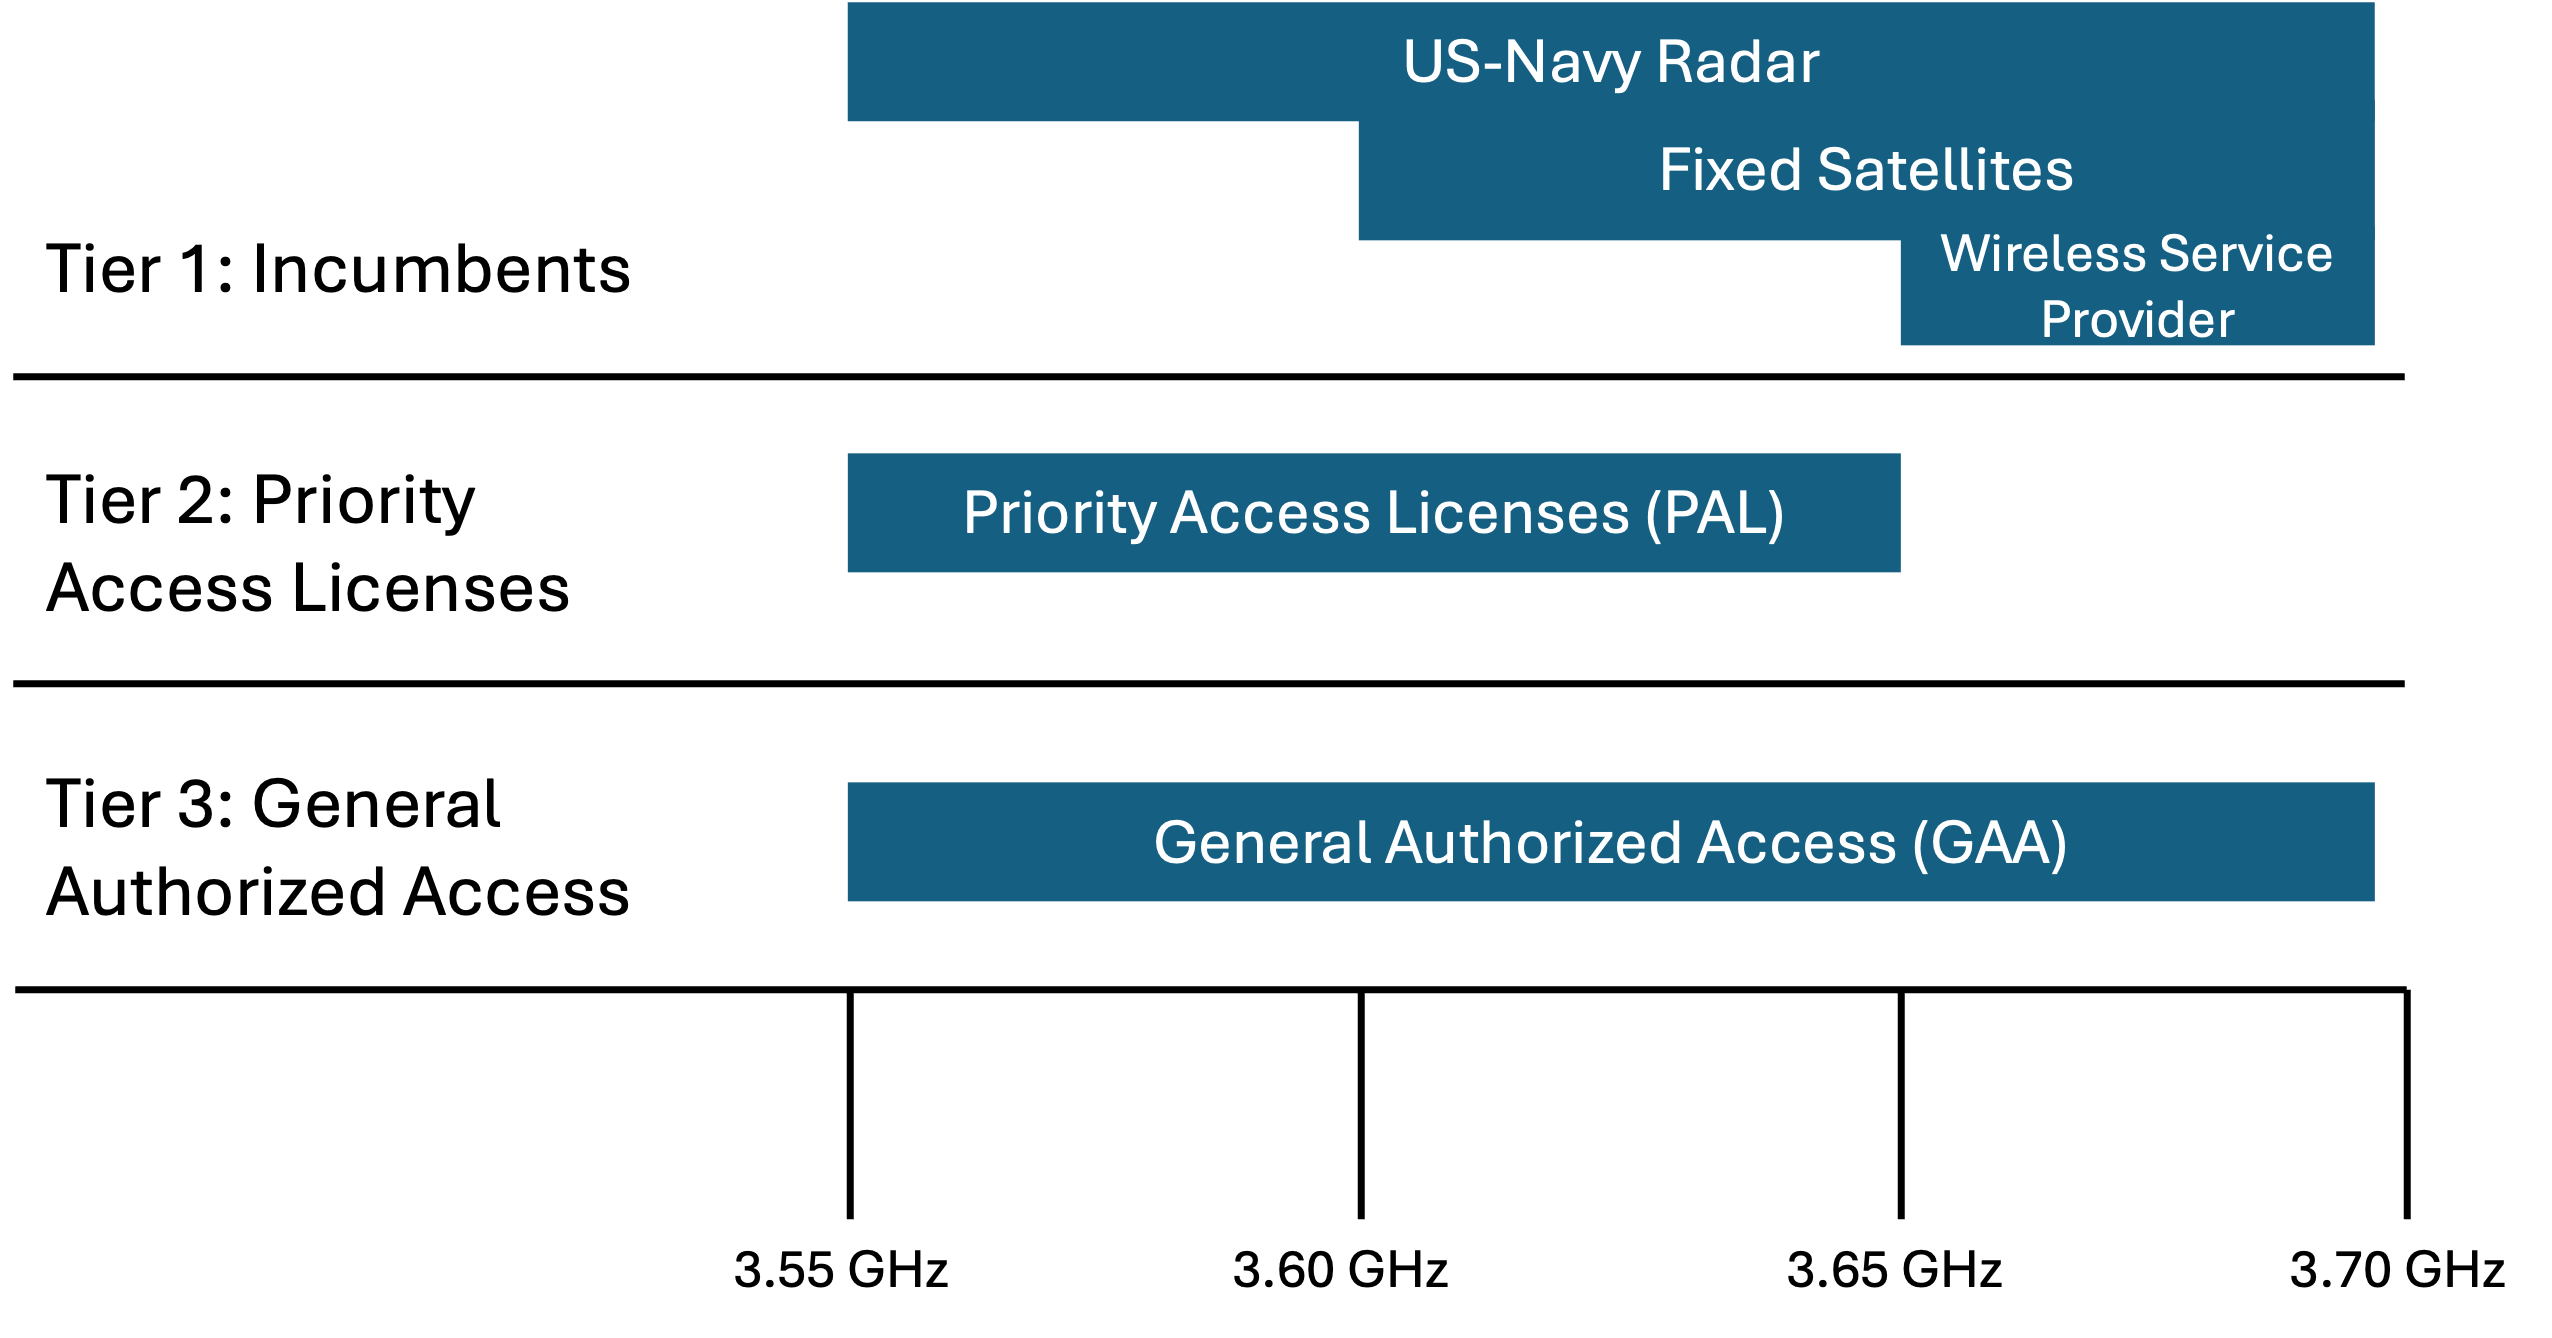
\includegraphics[width=\textwidth]{figures/cbrs_1.png}
\centering
\caption{The \gls{cbrs} spectrum }
\label{fig:cbrs-spectrum}
\centering
\end{figure}


Incumbent users include federal military radar systems and fixed satellite stations. These users have the highest priority and are granted uninterrupted access to the spectrum. Typically, these systems operate along coastal regions and require significant protection from interference.

\gls{pal} Users are licensed commercial users who acquire spectrum rights through an auction process. \gls{pal} licenses are granted for up to 10 MHz in a given geographic area and provide a level of protection from interference by lower-tier users. Common applications include private LTE/5G networks for enterprises, utilities, and healthcare.

\gls{gaa} users are the unlicensed users who can access the spectrum opportunistically in areas where it is not in use by Incumbent or \gls{pal} users.
\gls{gaa} users operate under strict rules to prevent interference with the higher-priority tiers. Figure 1.1 illustrates the three tiers of the \gls{cbrs} spectrum.

Since these tiers simultaneously use the \gls{cbrs} spectrum, the \gls{fcc} of the USA mandates that \gls{gaa} users must not cause interference with \gls{pal} or incumbent users, and \gls{pal} users must not cause interference with incumbent users. A \gls{sas} is used to manage the spectrum and avoid potential interference \cite{3}.

\gls{sas} is a cloud-based, automated frequency management system mandated by the \gls{fcc} to enforce \gls{cbrs} rules and ensure efficient use of the spectrum. \gls{sas} acts as a dynamic coordinator, regulating how the spectrum is shared and preventing interference between users across the three tiers.

The \gls{sas} continuously monitors the spectrum usage and allocates channels dynamically to users based on their tier. Incumbent users are always given precedence, followed by \gls{pal} users, and then \gls{gaa} users.
To prevent collision scenarios, particularly involving Incumbent users, \gls{sas} currently employs several mechanisms, including continuous monitoring, spectrum reallocation for non-priority users, and preemption for Incumbent users.

Preventing interference is crucial in \gls{cbrs} operations. \gls{sas} enforces a priority hierarchy, ensuring \gls{gaa} users access spectrum only when \gls{pal} and Incumbent users are inactive. If a higher-priority user requires access, \gls{sas} reallocates \gls{gaa} users dynamically. \gls{pal} users are similarly protected through exclusive spectrum assignments \cite{4}.  

\section{Background}

\gls{gan}s and diffusion-based generative models have gained significant traction for various applications, including spectrogram augmentation and audio synthesis. In \cite{14}, \gls{gan}-based models were employed for Radar spectrogram augmentation, leveraging a \gls{jdl} module for injecting diversity into synthetic data. While effective for enhancing dataset variability, the reliance on adversarial training often poses challenges in terms of stability and convergence, particularly in complex spectrogram domains.


The work in \cite{9} conducted a multimodal comparison of latent Diffusion Models (\gls{ddpm}s) and \gls{gan}s for medical image synthesis. Their results demonstrated the superiority of latent \gls{ddpm}s over Least Squares \gls{gan} and Variational Autoencoder \gls{gan}, particularly in generating high-quality, diverse images. While this comparison offers insights into the potential of diffusion models, its application was limited to medical imaging and did not address the challenges of dynamic spectrum scenarios, such as those found in \gls{cbrs}.

The U-Net architecture, proposed in Imagen \cite{16} and later adapted in \cite{17}, has shown promise for spectrogram-based high-quality audio synthesis. These approaches exploit the hierarchical encoding-decoding structure of U-Nets to generate fine-grained audio spectrograms but have not been extended to the domain of spectrum-sharing systems or collision detection in \gls{cbrs}.

Effective \gls{cbrs} management relies on robust collision detection, yet traditional rule-based methods struggle in dynamic environments due to scalability and adaptability challenges. Deep learning-based classification offers a promising alternative, but the scarcity of collision data limits training \cite{5}.  

To address this, we propose a novel spectrum-sharing system that generates spectrogram images of collision scenarios using \gls{gan} \cite{6}, \gls{ddpm} \cite{7}, and \gls{vq-vae} \cite{8}. These images will train a \gls{cnn} to detect collisions and alert \gls{sas}. 

We evaluate the generative models by comparing their impact on \gls{cnn} classification accuracy and data diversity. Then we simulate a \gls {cbrs} environment using MATLAB which uses \gls{drl} for instead of a \gls{sas} to assign channels to users in a rapidly changing environment. While \gls{gan}s and VAEs have been used to address data limitations, diffusion models have shown state-of-the-art results in natural image generation \cite{9}. However, a direct use generative AIs with \gls{cnn} for interference detection and \gls{drl} for channel allocation is unexplored.  

This work employs conditional \gls{gan}, conditional \gls{ddpm}, and \gls{vq-vae} models to generate visualized \gls{cbrs} datasets and compares their performance based on \gls{cnn} classification accuracy.  

The key contributions of this study are:
\begin{enumerate}
    \item Introduce a scalable and generalizable spectrum-sharing system for a dynamic \gls{cbrs} environment.
    \item Use Generative models to generate visualized waveforms of a \gls{cbrs} system.
    \item Make a quantitative comparison of three of the most popular generative models currently available, in generating frequency spectrogram images.
    \item Use \gls{drl} based channel allocation system with a \gls{cnn} based collision detection system to manage the \gls{cbrs} environment.
\end{enumerate}


This document consists of the following: Chapter 2 has the background explanations and the system architecture of this thesis and the Chapter 3 anaylze the results, performance of the genarative models and the \gls{drl} agent. Chapter 4 includes a discussion of the results and Chapter 5 includes the conclusion and future work.



%%%%%%%%%%%%%%%%
% Chapter 2
%%%%%%%%%%%%%%%%

\chapter{Methodology}
\label{chap:methods}

\section{Dataset}

The dataset utilized for training our generative models and the \gls{cnn} model was obtained from the research conducted by \cite{5} called the ViC dataset. This dataset comprises 2400 images belonging to 12 different scenarios for two channels. 

Each channel can have four possible states: empty, primary (RADAR), secondary (LTE), and collision. Since this spectrum-sharing system manages two tiers of users and two channels, there are 16 possible cases depending on how each user occupies each channel. However, four cases are discarded since the  \gls{cbsd} is assumed to use only one channel simultaneously. Thus, the two channels could be in 12 different states. Figure 2.1 illustrates the spectrogram images corresponding to the channel states across the 12 classes. We used 2000 images to train the generative models and the other 400 for the \gls{cnn} training. 

The class names presented in Figure 2.1 will be used throughout this paper when discussing the results. Waveforms were visualized using  Short Time Fourier Transform (STFT) with a size of $64 \times 64 $ matrix.

\begin{figure}[h]
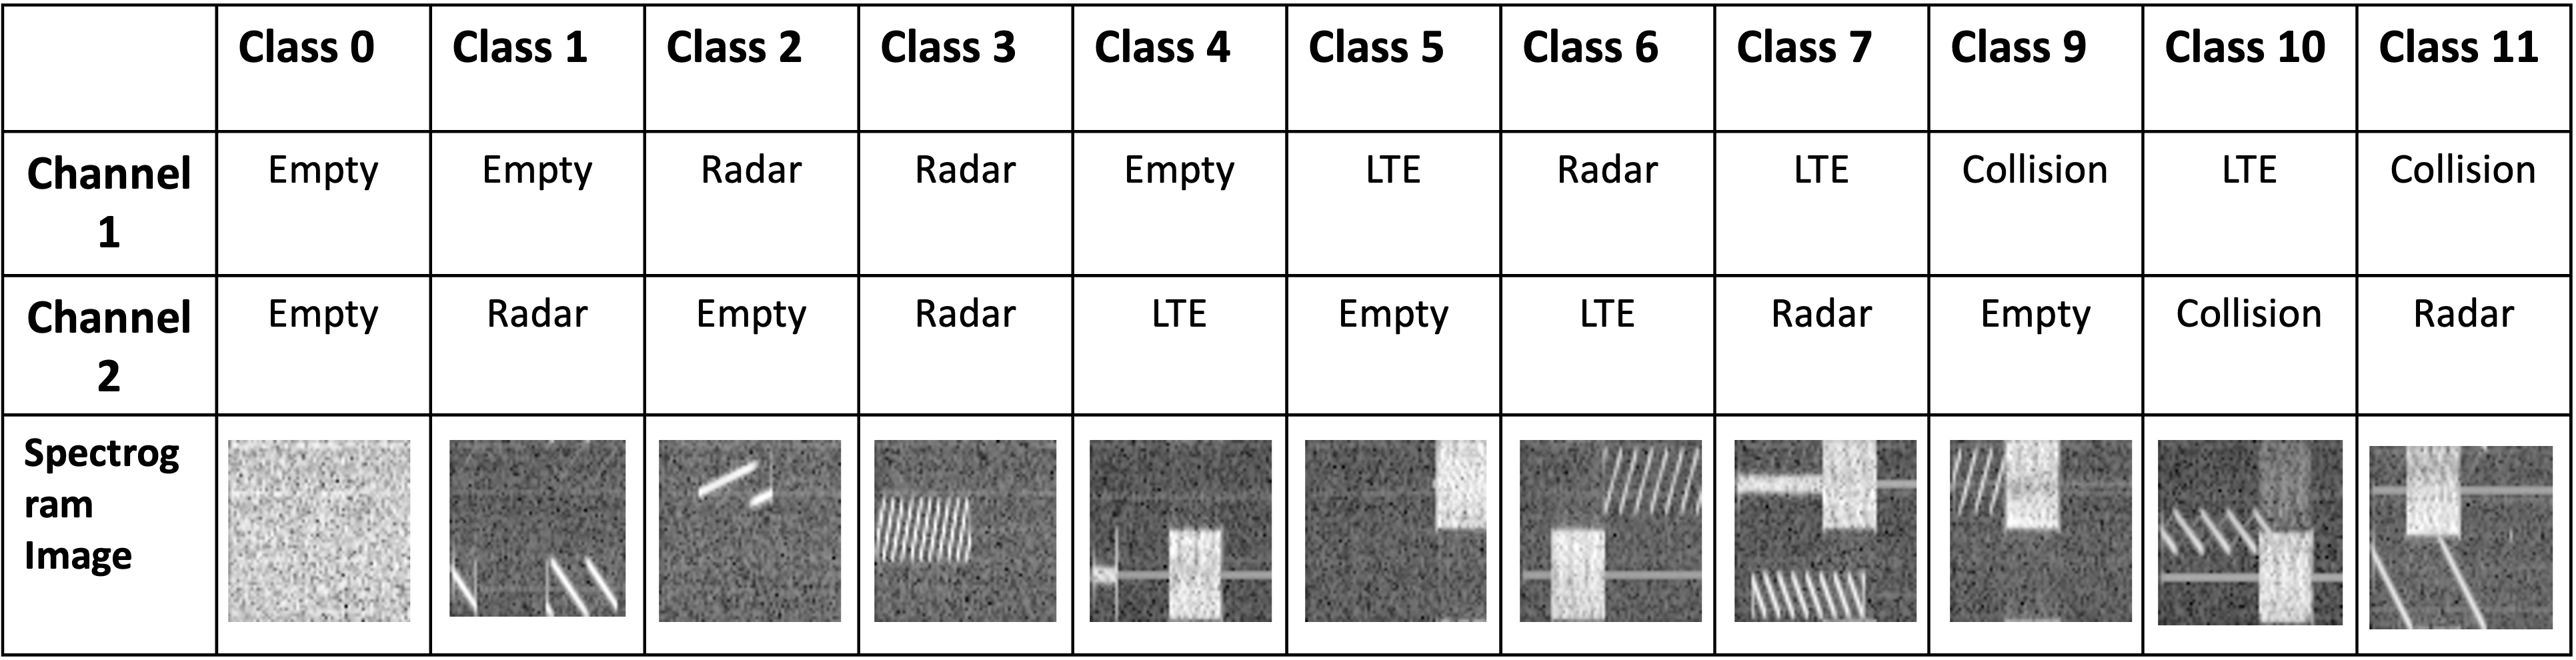
\includegraphics[width=\textwidth]{figures/classes_white_background.png}
\centering
\caption{Training ViC dataset containing the 12 classes \cite{5}}
\label{fig:training-dataset}
\centering
\end{figure}
%%%%%%%%%%%%%%%%%%%%%%%%%%%%%%%%%%%%%%%%%%%%%%%%%%%%%%%%%%%%%%%%%%%%%%%%%%%%%%%%%%%%%%%%%%%%%%%%%
\section{\gls{vq-vae}}

The \gls{vq-vae} is a generative model that combines continuous latent representations with discrete, interpretable codes by introducing a quantization mechanism. As illustrated in Figure 2.2 In \gls{vq-vae}, the encoder maps the input $x$ to a continuous latent representation $z_e(x)$ which is then quantized to the closest embedding $z_q(x)$ from a predefined discrete codebook ${e_1,e_2,...,e_k}$. This process ensures that the latent space is discrete and semantically meaningful. During training, the quantization mechanism minimizes the difference between $z_e(x)$ and $z_q(x)$ using a gradient-through approximation. The decoder then reconstructs the input $x$ from the quantized representation $z_q(x)$. The use of codebook ${e_1,e_2,...,e_k}$ enables the model to structure the latent space compactly, making it highly effective for tasks like image generation and speech synthesis. This discrete representation, denoted by $q(z|x)$, improves reconstruction quality by focusing on meaningful latent structures and allows efficient scaling for large datasets and complex generative tasks. The innovation of replacing continuous latent spaces with quantized embeddings results in a model that bridges the gap between interpretability and high-quality generation.

\begin{figure}[h]
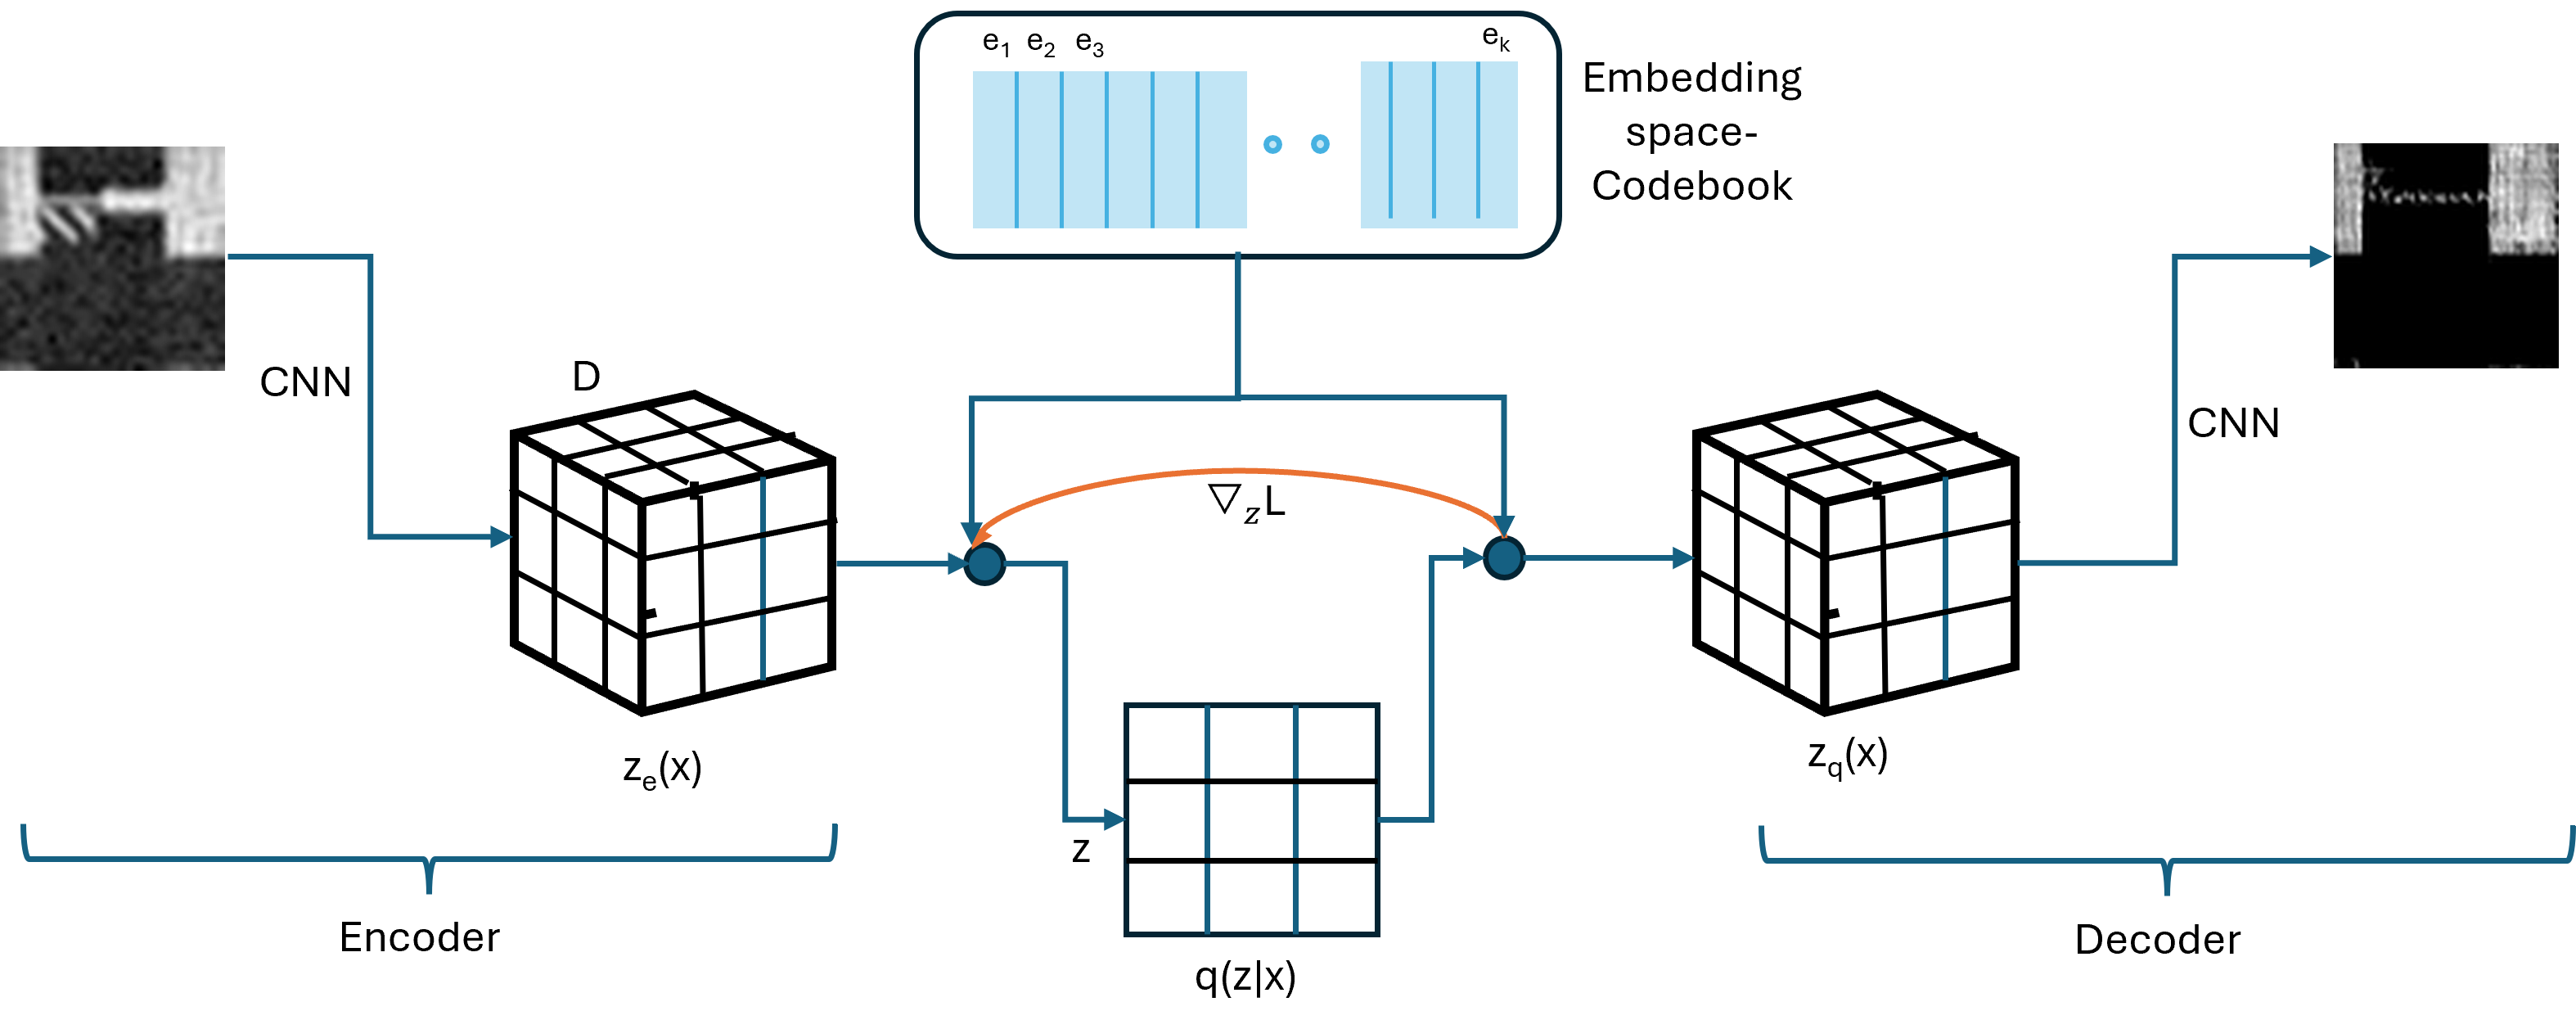
\includegraphics[width=\textwidth]{figures/vq-vae.png}
\centering
\caption{The \gls{vq-vae} architecture  }
\centering
\end{figure}


In the architecture of the conditional \gls{vq-vae} we used, the encoder is a \gls{cnn} designed to extract features from the input grayscale images. It has three convolutional layers to progressively reduce spatial dimensions while increasing the number of feature channels. The encoder also incorporates a residual stack, which consists of multiple residual layers to enhance feature extraction by allowing information to bypass intermediate transformations, thereby improving gradient flow and capturing complex patterns.

After encoding, the latent representation is passed through a 1x1 convolution layer to adjust the feature dimensions to match the input requirements of the vector quantizer.  This mapping is performed using the Euclidean distance between the latent vectors and the codebook embeddings. To ensure effective learning, the vector quantizer minimizes a combination of the reconstruction loss, a codebook commitment loss, and a latent quantization loss.
The loss function can be expressed as follows:
\begin{equation}
L = \mathbb{E}[\|x - \hat{x}\|^2] + \beta \cdot \mathbb{E}[\|z_{\text{enc}} - \text{sg}(z_{\text{quant}})\|^2]
\end{equation}

where $x$ is the input image, $\hat{x}$ is the reconstructed image, $z_{\text{enc}}$ is the latent vector from the encoder, $z_{\text{quant}}$ is the quantized vector, and $\text{sg}(\cdot)$ denotes the stop-gradient operator.

The decoder is another \gls{cnn} that takes the quantized latent representations and reconstructs the original input images. It mirrors the encoder's structure, starting with a convolutional layer followed by the residual stack to refine features, and ends with transposed convolutional layers to upsample the latent representation back to the original input dimensions. The decoder ensures that the reconstructed images retain high fidelity to the input.

We implemented a conditional \gls{vq-vae} model, enabling class-specific image generation. The encoder compresses grayscale input images using three convolution layers followed by residual blocks, while the decoder mirrors this process using transposed convolutions to reconstruct the data. The quantization layer is also class-conditioned, leveraging a codebook with 512 embeddings, each of 64 dimensions. 

%%%%%%%%%%%%%%%%%%%%%%%%%%%%%%%%%%%%%%%%%%%%%%%%%%%%%%%%%%%%%%%%%%%%%%%%%%%%%%%%%%%%%%%%%%%%%%%%%
\section{\gls{gan}}

\gls{gan}s, consist of two neural networks: a generator that creates data samples and a discriminator that evaluates their authenticity. The generator and discriminator engage in a game-theoretic scenario where the generator aims to produce indistinguishable fake data, while the discriminator strives to identify real from generated data. This adversarial process allows \gls{gan}s to produce highly realistic images, audio, and other data forms \cite{10}. The loss functions used by the Generator and the Discriminator can be written as follows. Figure 2.3 illustrates this architecture.
\begin{figure}[h]
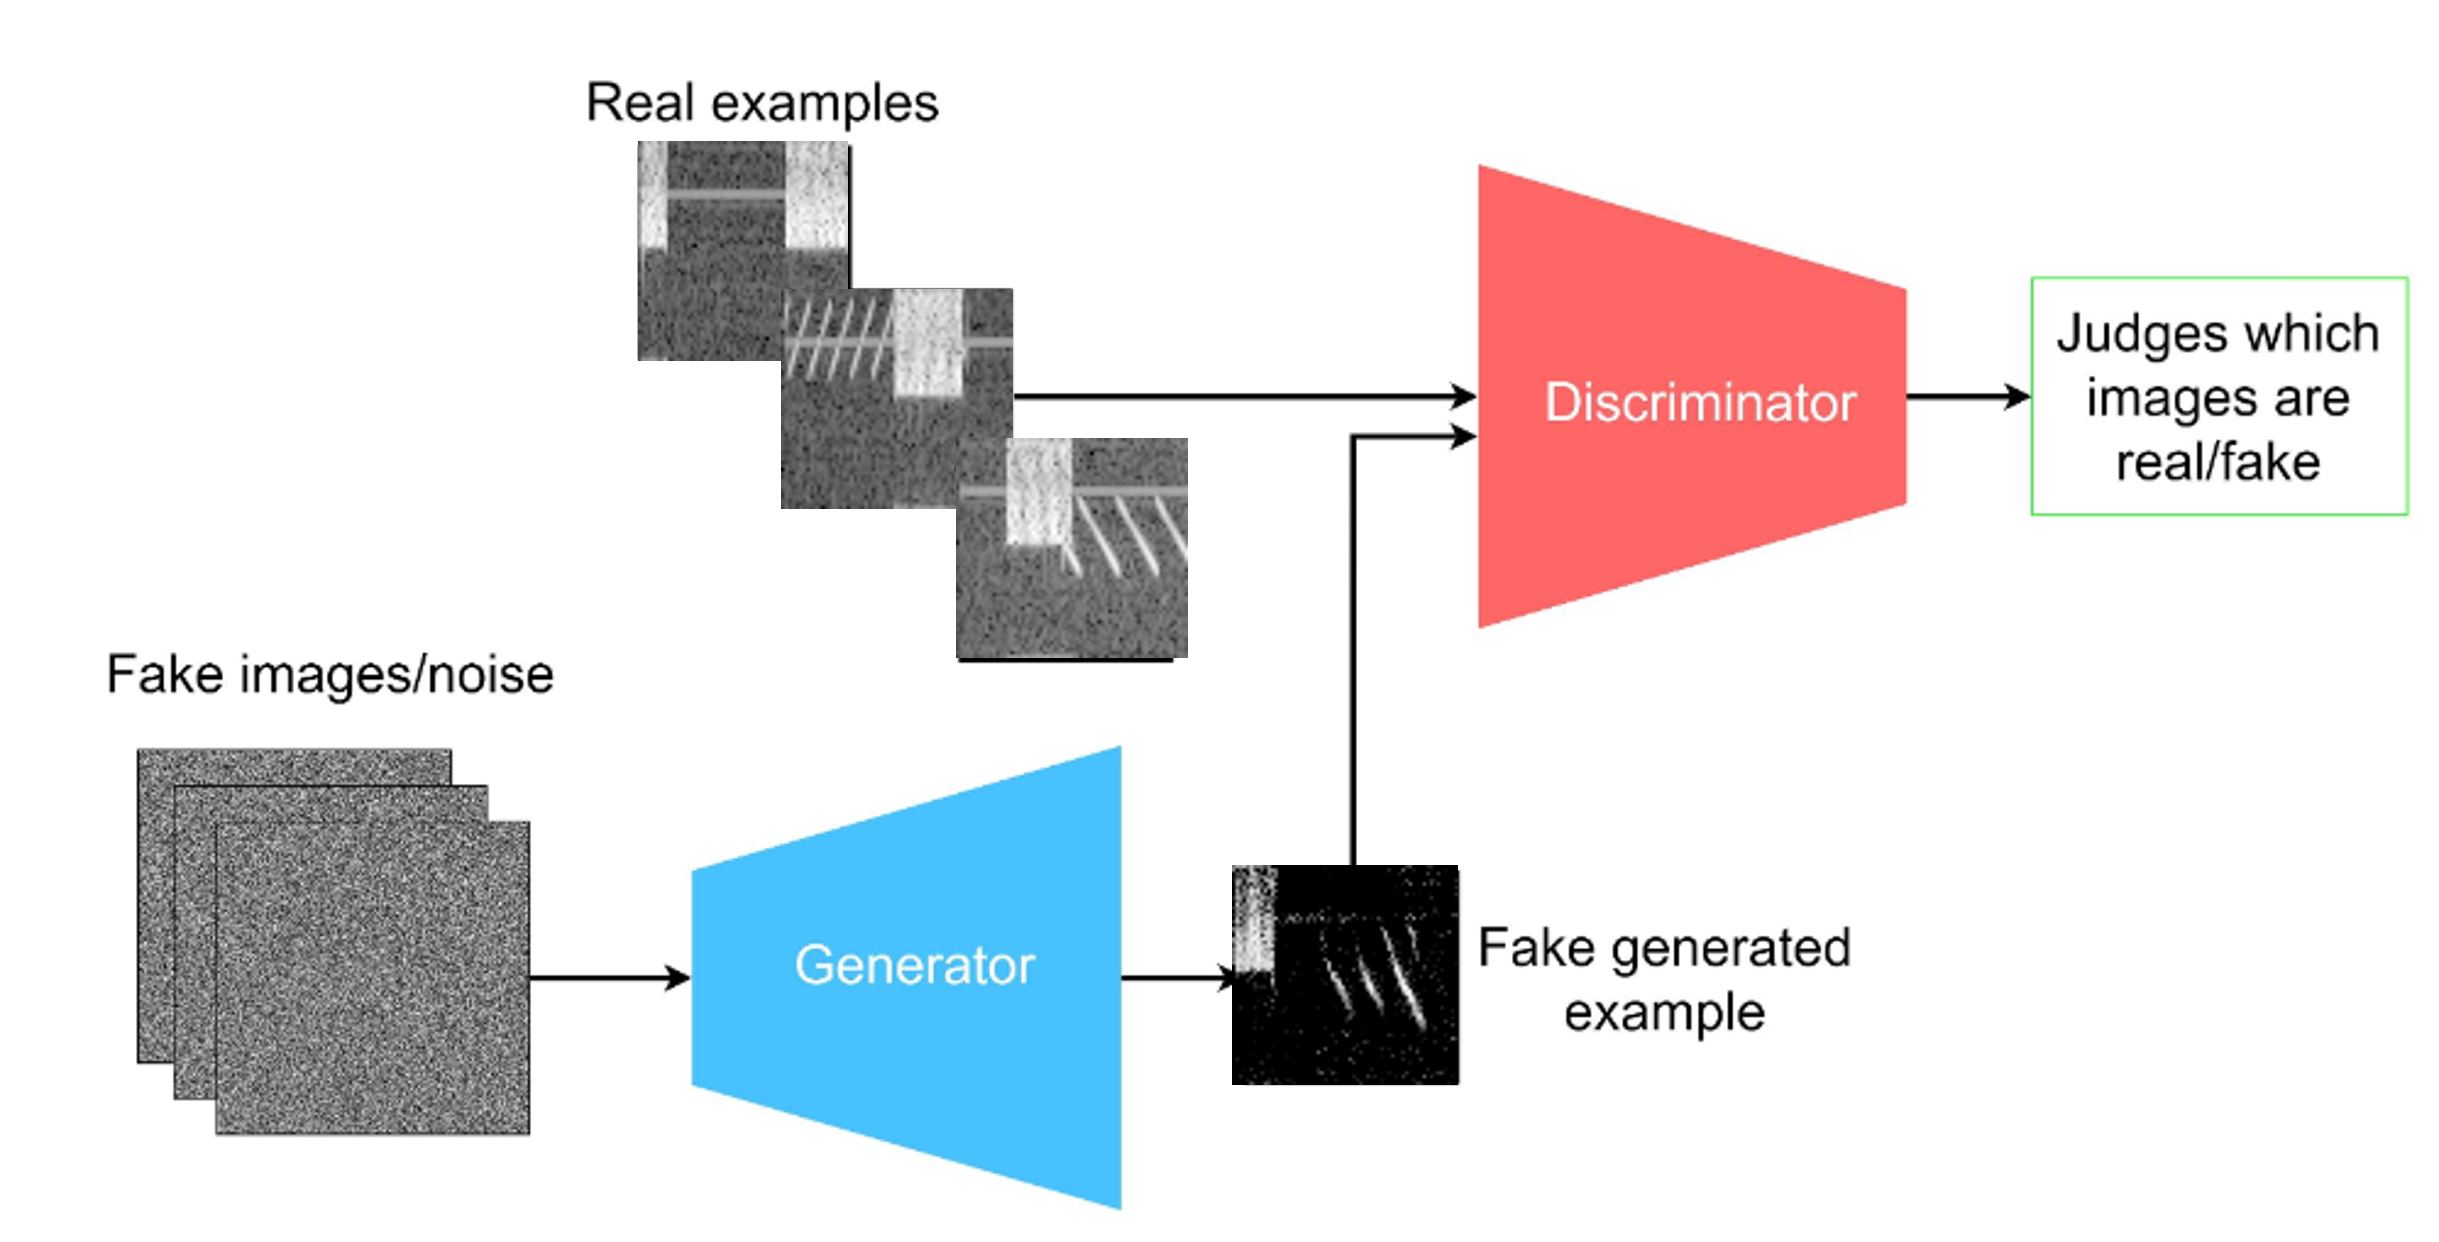
\includegraphics[width=9cm]{figures/gan.png}
\centering
\caption{The \gls{gan} architecture  }
\centering
\end{figure} 
 $L_D$ and $L_G$ are the loss functions for the Discriminator and the Generator for image $x$, respectively.
\begin{equation}
    L_D=\mathbb{E}[max(0,1 - D(x_{real}))]+\mathbb{E}[max(0,1+D(G(z_{fake})))]
\end{equation}

\begin{equation}
    L_G=\mathbb{E}[D(G(z_{fake}))]
\end{equation}

We used a conditional \gls{gan} with a Generator $\mathcal{G}$ and a Discriminator $\mathcal{D}$ which were trained simultaneously through a min-max game. For the Generator, we used an input noise vector $z$ of 100 dimensions and an embedding layer to convert class labels into embeddings with five convolution layers and ReLU activations in hidden layers. Tanh activation was used in the output layer to produce pixel values in the range [-1, 1]. In the Discriminator, five convolution layers were used to down-sample the images with Leaky ReLU activations in hidden layers. We used Sigmoid activation in the output layer to produce the probability.
\begin{figure}[h]
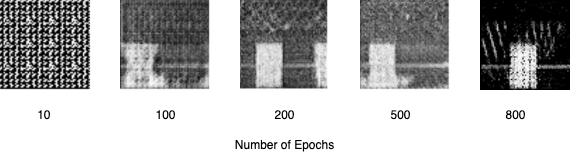
\includegraphics[width=9cm]{figures/gan training.drawio (1).png}
\centering
\caption{Spectrogram images generated by the Generator of the \gls{gan}}
\centering
\end{figure}

We generated 1200 images with 100 images per class for the twelve classes and used the pre-trained \gls{cnn} model to classify the images. 

%%%%%%%%%%%%%%%%%%%%%%%%%%%%%%%%%%%%%%%%%%%%%%%%%%%%%%%%%%%%%%%%%%%%%%%%%%%%%%%%%%%%%%%%%%%%%%%%%
\section{\gls{ddpm}}

\gls{ddpm}s are generative models designed for image generation using variational inference. They operate through a Markovian process that involves a finite sequence of steps, denoted as $T$. Training involves two main stages: the forward process, where noise is added to data in a controlled manner, and the reverse process, where the model learns to denoise this data step-by-step. Each step in this process acts as a denoising operation, aiming to refine the image quality progressively\cite{7}. Figure 2.5 illustrates the diffusion process of the \gls{ddpm}. 

\begin{figure}[h]
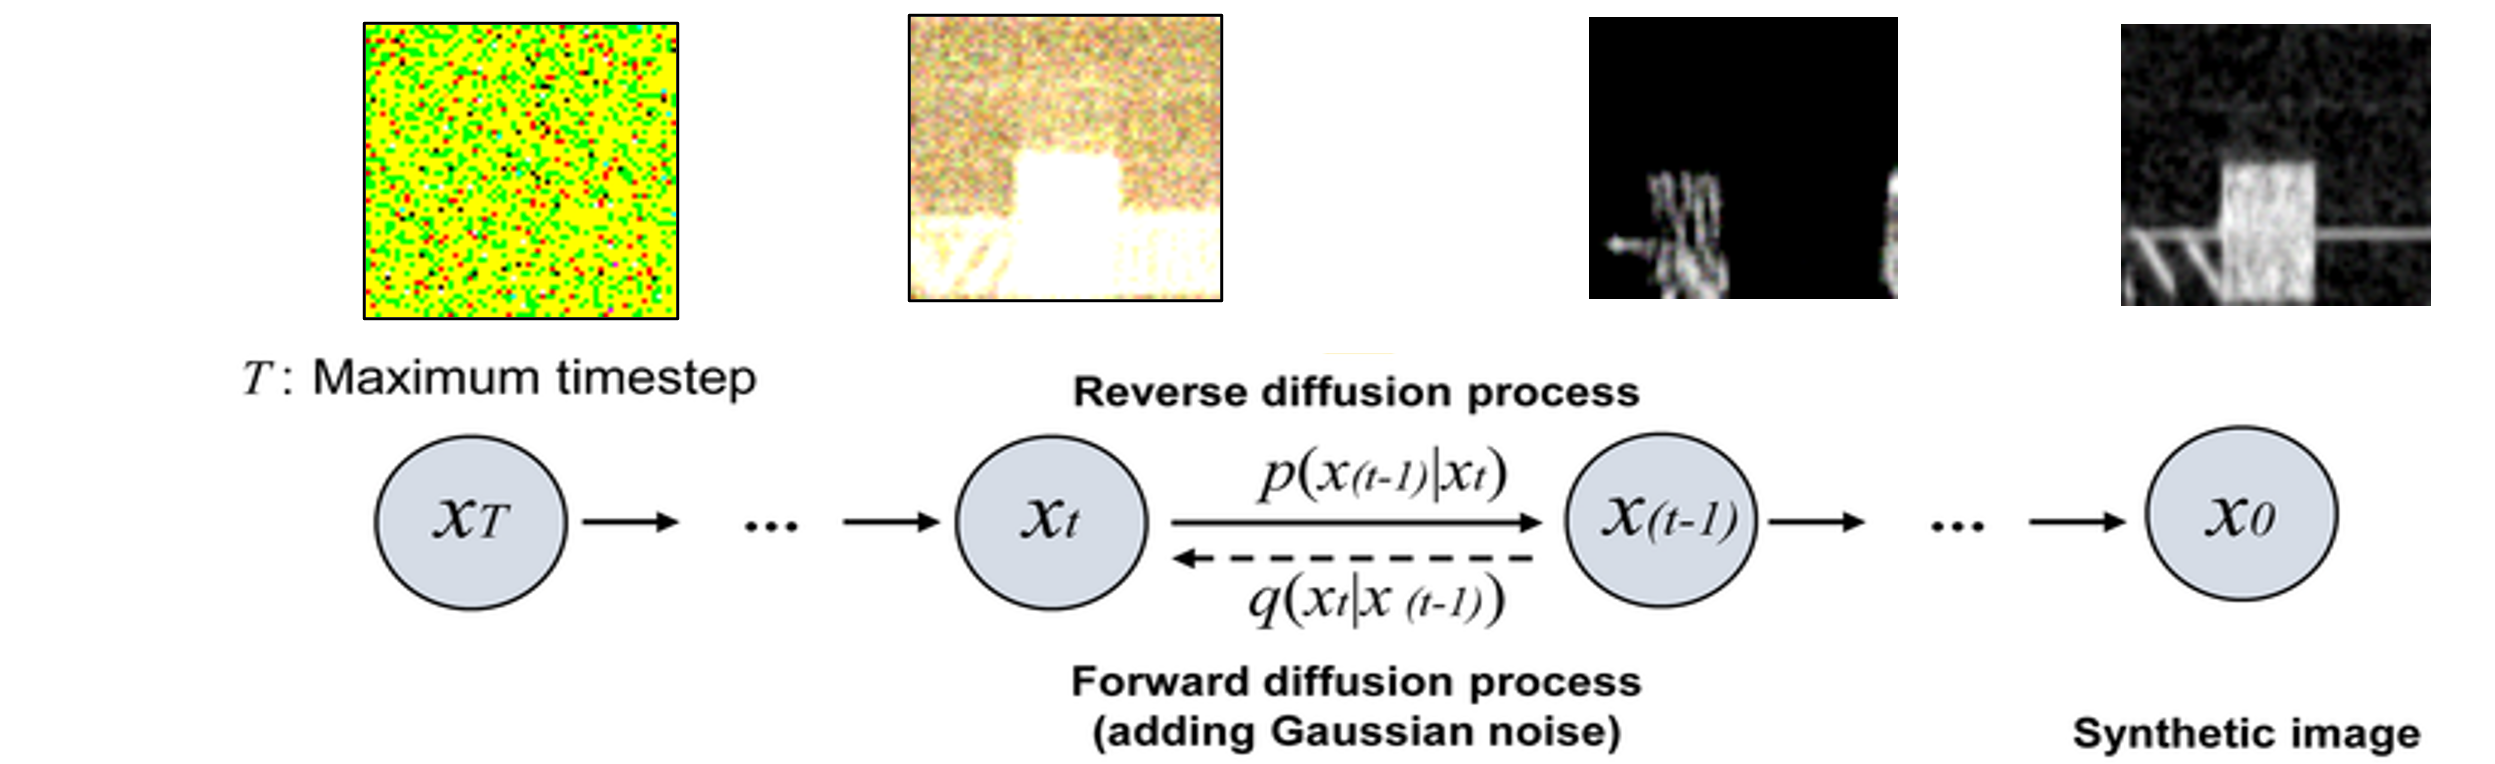
\includegraphics[width=\textwidth]{figures/ddpm.png}
\centering
\caption{ Diffusion process of the \gls{ddpm}}
\centering
\end{figure}

During the forward process, the clean image $y_0$ is sampled with Gaussian noise of variance ${\beta_1,....,\beta_T}$ is added over $T$ time steps.
\begin{equation}
\begin{split}
    q(y_t\mid y_0) :=\mathcal{N}(y_t;\sqrt{\bar{\alpha_t}}y_0,(1-\bar{\alpha_t})I)\\
    =\sqrt{\bar{\alpha_t}}y_0+\epsilon\sqrt{1-\bar{\alpha_t}},\epsilon \sim \mathcal{N}(0,I)
    \end{split}
\end{equation}
Where $\alpha_t=1-\beta_t$

In the reverse process, the added noise is removed step by step to recover the image $y_0$.
\begin{equation}
    p(y_T)=\mathcal{N}(0,I)
\end{equation}
\begin{equation}
    p(y_{(t-1)}\mid y_t)=\mathcal{N}(y_{(t-1)};\mu_{\theta}(y_t,t),\sqrt{\beta_t}I)
\end{equation}

We used a conditional \gls{ddpm}, and when training the \gls{ddpm} we enabled mixed precision training and multithreaded data loaders. We sampled the images regularly during the training and we could see the learning rate gradually decreasing with the time steps. 
For training our model we sampled a timestep $t\sim U[1,T]$ with $T=2000$ and a $5\times10^{-3}$ learning rate.
After training the model, we used the trained weights to generate 1200 images with 100 images per class and used the pre-trained \gls{cnn} model to classify the images to their respective classes. 
\begin{figure}[h]
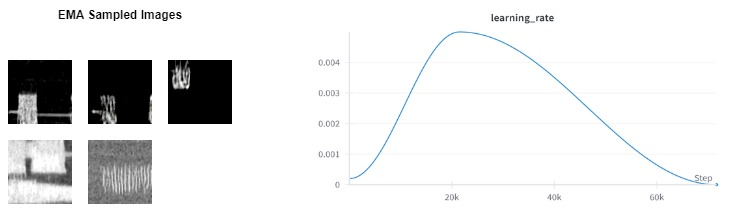
\includegraphics[width=\textwidth]{figures/ema_learning_rate.jpg}
\centering
\caption{EMA sampled images and the change of the learning rate with each time step when training the \gls{ddpm} }
\centering
\end{figure}
%%%%%%%%%%%%%%%%%%%%%%%%%%%%%%%%%%%%%%%%%%%%%%%%%%%%%%%%%%%%%%%%%%%%%%%%%%%%%%%%%%%%%%%%%%%%%%%%%
\section{\gls{cnn}}
\gls{cnn}s are a type of deep learning model widely used for image analysis tasks. They are designed to automatically and adaptively learn spatial hierarchies of features from input data through layers of convolutional filters. These filters detect patterns such as edges, textures, and more complex features in the images, making \gls{cnn}s highly effective for tasks like image classification.


We trained a \gls{cnn} model that can detect collision scenarios using the generated spectrogram data from the three models. 
Since the spectrogram images generated by the \gls{ddpm}, \gls{gan}, and \gls{vq-vae} models contained some noise, which could have led to misclassification by conventional \gls{cnn} architectures, particularly when distinguishing fine-grained features,  we employed an enhanced \gls{cnn} architecture specifically designed to effectively capture and differentiate subtle details within the images, thereby mitigating the impact of noise on classification accuracy.

We used a \gls{cnn} architecture based on a modified ResNet-50 model, enhanced with a \gls{cbam} to improve its feature extraction and classification capabilities. The architecture comprised convolutional layers for basic feature extraction, residual blocks for efficient gradient propagation, \gls{gap} for summarizing spatial information, and a \gls{fc} layer adapted for classifying the 12 spectrogram image classes.

The model was trained on spectrogram images resized to 448×448 for capturing finer details. The training used the Adam\cite{18} optimizer for adaptive gradient updates and a learning rate scheduler that reduced the learning rate every five epochs to ensure stable convergence.  

%%%%%%%%%%%%%%%%%%%%%%%%%%%%%%%%%%%%%%%%%%%%%%%%%%%%%%%%%%%%%%%%%%%%%%%%%%%%%%%%%%%%%%%%%%%%%%%%%
\section{\gls{drl}}

In this work, we employed a \gls{drl} agent to learn optimal spectrum access strategies in a simulated \gls{cbrs} environment. The agent interacts with an environment that mimics the dynamic characteristics of the CBRS band, including incumbent radar signals and LTE-based priority access users. The environment is modeled as a Markov Decision Process (MDP) where the agent observes the occupancy of two communication channels and selects an action from a discrete set: idle, use channel 1, or use channel 2.

We implemented a \gls{dqn} agent that approximates the Q-value function using a neural network. The agent receives as input a two-dimensional observation vector representing the current channel state, where each element indicates whether a channel is occupied (1) or free (0), as predicted by the pre-trained \gls{cnn} model that analyzes the spectrogram of the received signal. The agent’s goal is to maximize a cumulative reward by learning a policy that avoids interference with higher-tier users while efficiently utilizing the available spectrum. The reward structure is defined such that selecting an idle channel yields a positive reward, selecting an occupied channel results in a penalty, and remaining idle results in a small negative reward to discourage inactivity.

The neural network used by the DQN agent consists of a feature input layer followed by two fully connected layers with ReLU activations, and a final output layer that estimates Q-values for each possible action. During training, we enabled GPU acceleration to improve performance. The training utilized an experience replay buffer and a target network, and was configured with Double DQN and a smooth target update factor of $10^{-3}$ to stabilize learning. We set the discount factor $\gamma=0.99$, and trained the model for 1000 episodes with a maximum of 100 steps per episode.

The environment generates new signal observations by randomly simulating different channel conditions, including ‘empty’, ‘radar’, ‘LTE’, and ‘collision’. These synthetic signals are converted into spectrogram images, resized to 224$\times$224 pixels, and classified by the CNN. This predicted class is used to update the channel occupancy vector, which forms the observation space for the DRL agent.
%%%%%%%%%%%%%%%%%%%%%%%%%%%%%%%%%%%%%%%%%%%%%%%%%%%%%%%%%%%%%%%%%%%%%%%%%%%%%%%%%%%%%%%%%%%%%%%%%
\section{System Architecture}

We evaluated classification performance across different generative models and computed class-wise and overall accuracy, along with \gls{fid} scores for each class. Then, we used a pre-trained CNN model trained with a dataset comprising both original data and the data generated by the three generative models to detect incumbent users. Figure 2.7 illustrates this scenario.
\begin{figure}[h]
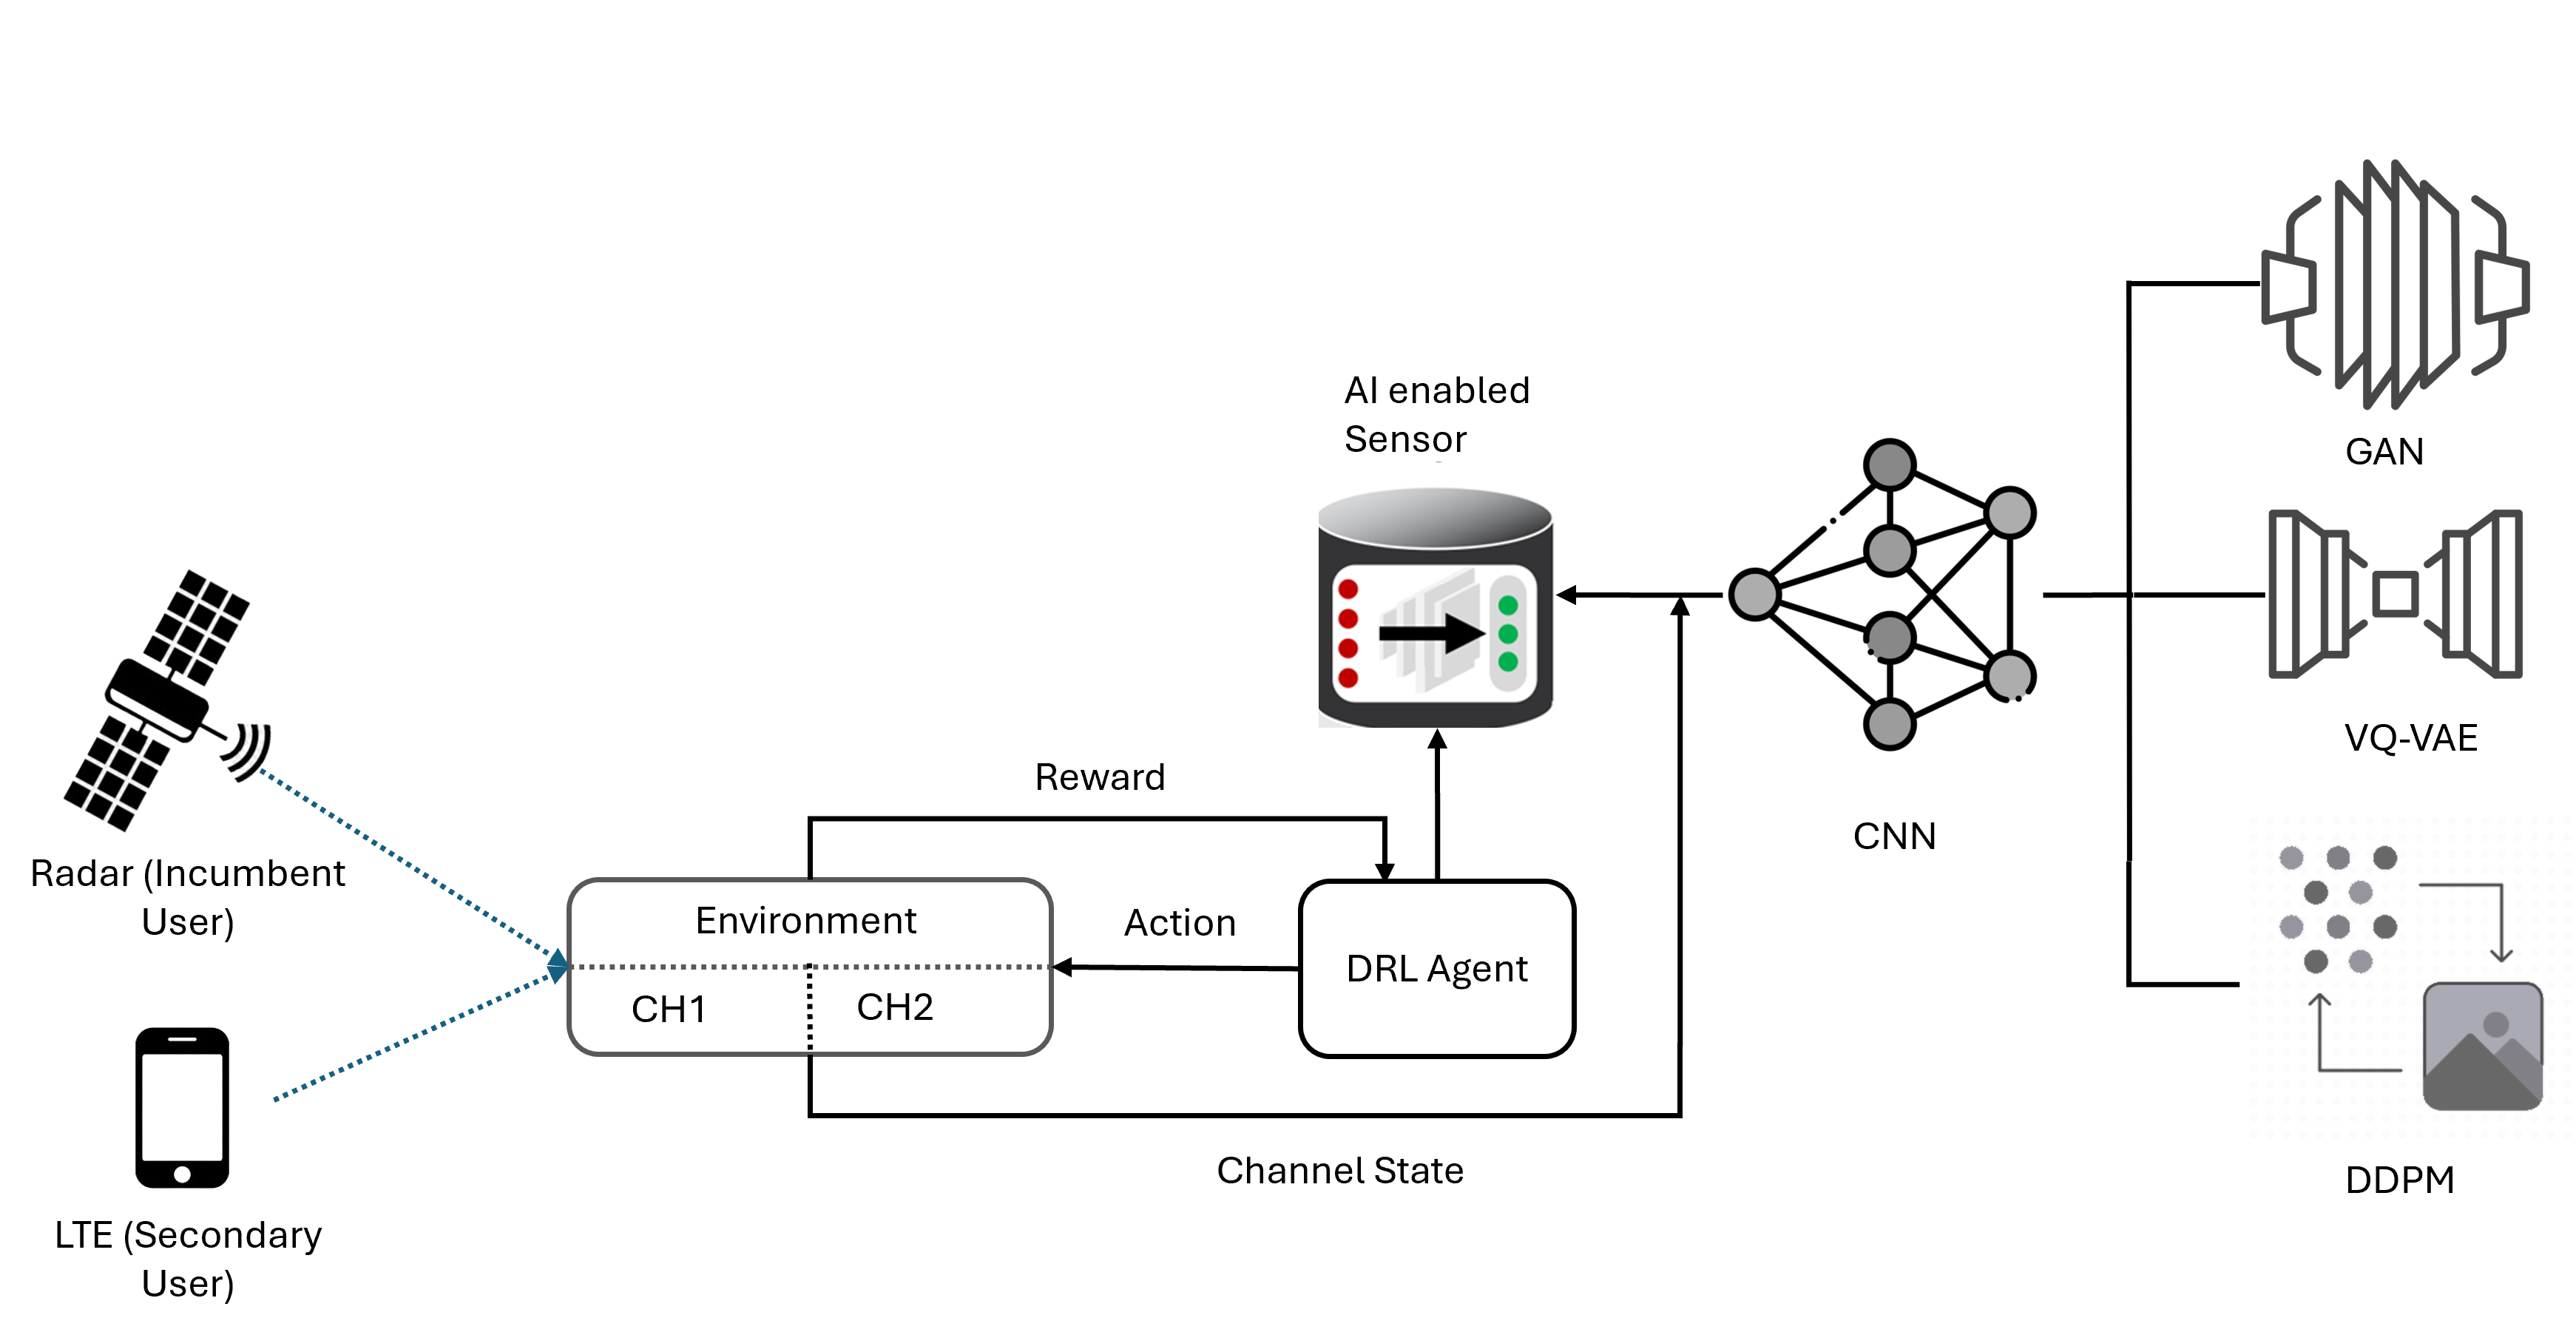
\includegraphics[width=\textwidth]{figures/system-architecture.png}
\centering
\caption{ System Architecture}
\centering
\end{figure}

\section{Experimental Setting}
\subsection{\gls{vq-vae}}
The conditional \gls{vq-vae} model was designed for class-specific image generation, with an encoder that compresses grayscale inputs through three convolutional layers and residual blocks to enhance feature extraction. The quantization layer, class-conditioned, uses a codebook of 512 embeddings (64 dimensions each) to discretize the latent space. A 1×1 convolution adjusts the encoder's output to fit the quantizer's input requirements. The decoder, structured similarly to the encoder, uses transposed convolutions and residual stacks to reconstruct high-fidelity images from quantized representations. The model generated 1,200 images, with 100 per class across 12 classes, which were classified using a pre-trained \gls{cnn}.

\subsection{\gls{gan}}
The conditional \gls{gan} used in this study consists of a generator and discriminator trained in a min-max game. The generator takes a 100-dimensional noise vector and class embeddings, passing them through five convolutional layers with ReLU activations and a Tanh output to generate pixel values in the range [-1, 1]. The discriminator uses five convolutional layers with Leaky ReLU activations to downsample input images, and a Sigmoid output provides a probability score. The model generated 1,200 images, with 100 per class across 12 classes, which were classified using a pre-trained \gls{cnn}.

\subsection{\gls{ddpm}}
The conditional \gls{ddpm} used in this study generates images through a two-stage Markovian process: a forward process, where Gaussian noise is added to the clean image over T=2000 timesteps, and a reverse process, where the model removes the noise step-by-step to reconstruct the original image. Mixed precision training and multithreaded data loaders were utilized for efficiency, and images were sampled during training to monitor progress. The model was trained with a learning rate of $5\times10^{-3}$, sampling timesteps $t\sim U[1,T]$ After training, 1,200 images (100 per class) were generated and classified using a pre-trained \gls{cnn}.

\subsection{\gls{cnn}}
A modified ResNet-50 architecture with a \gls{cbam} was used to classify 12 spectrogram image classes, effectively capturing fine-grained details despite noise. The model was trained on 448×448 resized images using the Adam optimizer and a learning rate scheduler to ensure stable convergence. For training, we used a combination of the original dataset and the generated data from each model. The combined dataset was divided into 80\% for training and 20\% for inference, and the results are based on three separately trained models, each incorporating generated data from one of the three-generation models.

We compared the class-wise and overall accuracy of the \gls{cnn} classification model trained with data generated by different models for the inference set. Then, we calculated the \gls{fid} score for each class. 

\subsection{\gls{fid}}
\gls{fid} is a widely used metric for evaluating the quality of images generated by generative models. It quantitatively compares the distributions of features extracted from real and generated images in a high-level feature space. These features are typically obtained from a pre-trained neural network, such as the Inception-v3 model. The \gls{fid} score is lower when the two distributions are closer, indicating higher quality and diversity of the generated images [21].

Let $\mu_r$ and $\Sigma_r$ represent the mean and covariance of the features extracted from real images, and $\mu_g$ and $\Sigma_g$ represent the mean and covariance of the features extracted from generated images. The \gls{fid} score is calculated using the following formula:

\begin{equation}
\text{FID} = \|\mu_r - \mu_g\|_2^2 + \text{Tr}(\Sigma_r + \Sigma_g - 2 (\Sigma_r \Sigma_g)^{\frac{1}{2}})
\end{equation}

Usually, to compute the \gls{fid}, real and generated images are passed through the pre-trained Inception-v3 network, and features are extracted from a specific layer (often the "pool3" layer). The means and covariances of these features are then computed for both datasets. However, in this paper, we used a ResNet18 model with the final classification layer replaced instead of Inception-v3.  The ResNet18 model employed for \gls{fid} calculation is distinct from the \gls{cnn} model used for classification. While the ResNet18 was trained exclusively on the original dataset to extract consistent feature representations for real and generated images, the classification \gls{cnn} was trained on a combined dataset comprising both real and synthetic data. This separation ensures that the \gls{fid} evaluation remains unbiased by the influence of synthetic data used in the classification task. Finally, the \gls{fid} score is calculated by substituting these statistics into equation 2.7. 

A lower \gls{fid} Score indicates that the distributions of real and generated features are more similar, implying better quality and diversity of generated images whereas a higher \gls{fid} score indicates that the generated images are less similar to real images, suggesting poorer quality or lack of diversity.

\subsection{\gls{pca}}
\gls{pca} is a statistical technique used for dimensionality reduction, facilitating the analysis and visualization of high-dimensional data. By transforming the original variables into a new set of uncorrelated variables, \gls{pca} captures the directions of maximum variance in the data. The first principal component accounts for the largest possible variance, with each succeeding component accounting for the remaining variance under the constraint of being orthogonal to the preceding components. This method simplifies complex datasets while preserving their essential patterns and structures \cite{12}.

\subsection{\gls{drl}}
The \gls{drl} agent observes the current state (e.g., channel occupancy or spectrogram predictions), selects an action (e.g., choose Channel 1, Channel 2, or remain idle), and receives a reward based on the outcome (e.g., successful transmission or interference avoidance). Over repeated episodes, the agent learns to maximize its long-term performance, such as throughput or interference avoidance, by training a neural network to approximate optimal policies. 

%%%%%%%%%%%%%%%%
% Chapter 3
%%%%%%%%%%%%%%%%

\chapter{Results}
\label{chap:results}
\begin{figure}[h!]
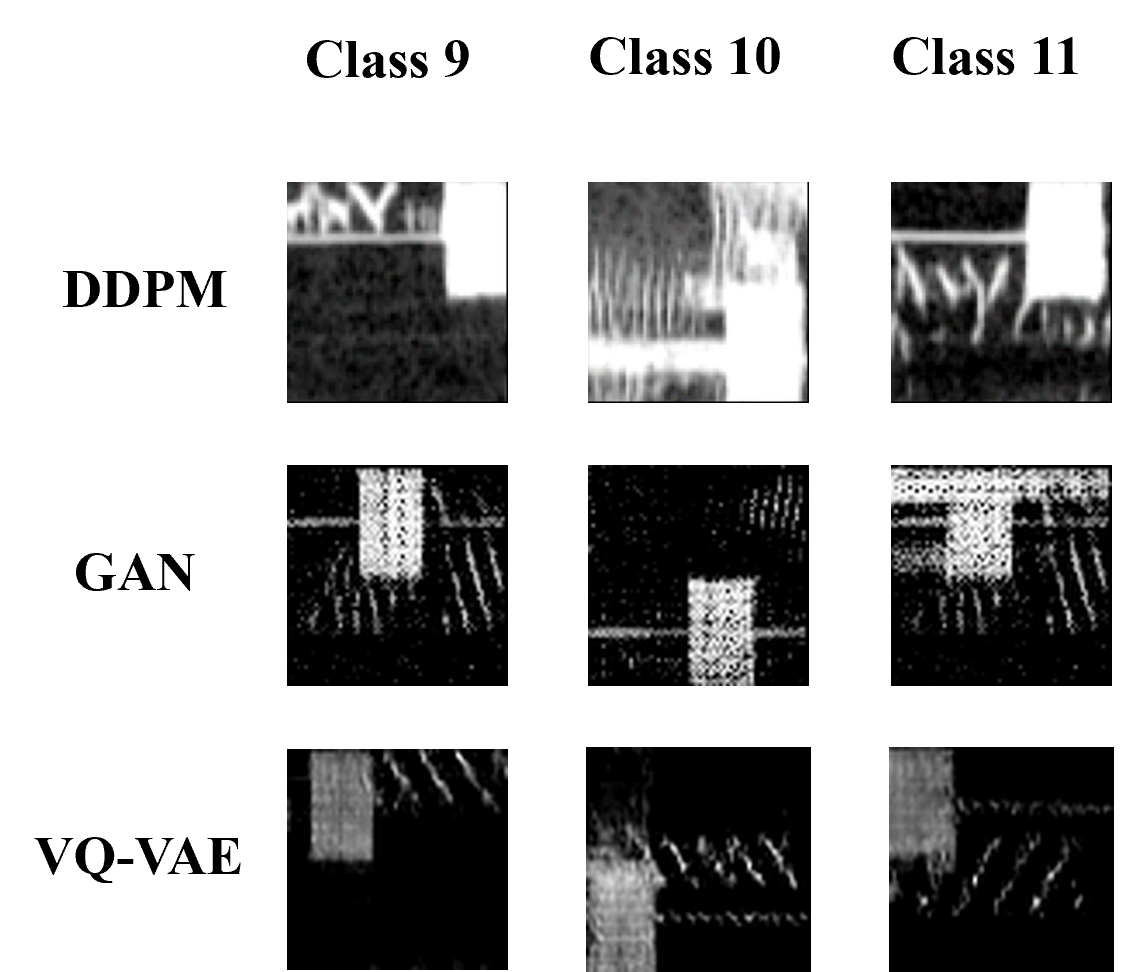
\includegraphics[width=10cm]{figures/Picture7.png}
\centering
\caption{A side-by-side comparison of some of the collision scenarios generated by the \gls{ddpm}, the \gls{gan}, and the \gls{vq-vae} }
\centering
\end{figure}

Classes depicted in Figure 3.1: class 9, class 10, and class 11 are all collision scenarios (Refer to Figure 2.1), which were generated by the \gls{ddpm}, the \gls{gan}, and the \gls{vq-vae}. 

\begin{figure*}[ht]
    \centering
    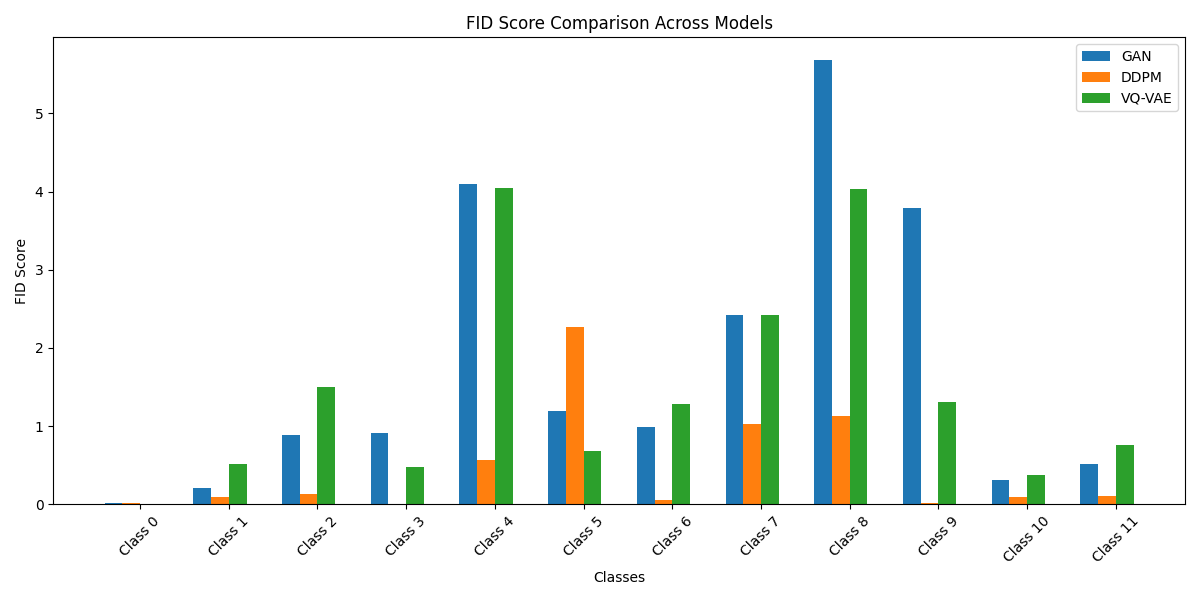
\includegraphics[width=\textwidth]{figures/Figure_12.png} 
    \caption{\gls{fid} Score Comparison Across Models for Different Classes.}
    \label{fig:fid_scores}
\end{figure*}
Figure 3.2 illustrates the change in \gls{fid} score across the classes for the 3 models.  The \gls{gan}, \gls{ddpm}, and \gls{vq-vae} models achieved average \gls{fid} scores of 1.944, 0.504, and 1.580, respectively. We used a ResNet18 model with the final classification layer replaced to extract features instead of using a pre-trained InceptionV3 network due to the specific nature of our dataset.

Since our dataset lacks the complex textures, patterns, and color information typically found in natural image datasets, the differences between real and generated spectrograms are smaller in the feature space. As a result, the \gls{fid} scores we obtained are smaller than usual for all three models.

Class 0 consistently shows near-zero \gls{fid} scores across all three models due to its purely noise-like nature. As observed in the graph, the classes representing collision scenarios—Class 9, Class 10, and Class 11—exhibit significantly lower \gls{fid} scores for images generated by the \gls{ddpm}. This suggests that the spectrogram images with collision scenarios generated by the \gls{ddpm} are more natural and resemble the original dataset better than the other two models. The other two models also have relatively low \gls{fid} scores for Class 10 and Class 11.

Among the three models, the \gls{ddpm} also has the lowest average \gls{fid} score, suggesting that \gls{ddpm} is the most effective model overall for generating spectrograms that closely resemble the real dataset, as evidenced by its consistently low \gls{fid} scores across most classes.

The \gls{gan} model's high \gls{fid} scores across many classes suggest model collapse in its generated spectrograms for this dataset, to which \gls{gan}s are susceptible. Given that our main focus is on generating a diverse dataset to improve the accuracy of a visualized interference classification system, having a wide variety of data is essential.

\gls{vq-vae} model, on the other hand, shows varied performance, outperforming \gls{gan} in many cases (e.g., Classes 1, 2, 6, 9) but falling behind \gls{ddpm} in most.

\begin{figure}[h]
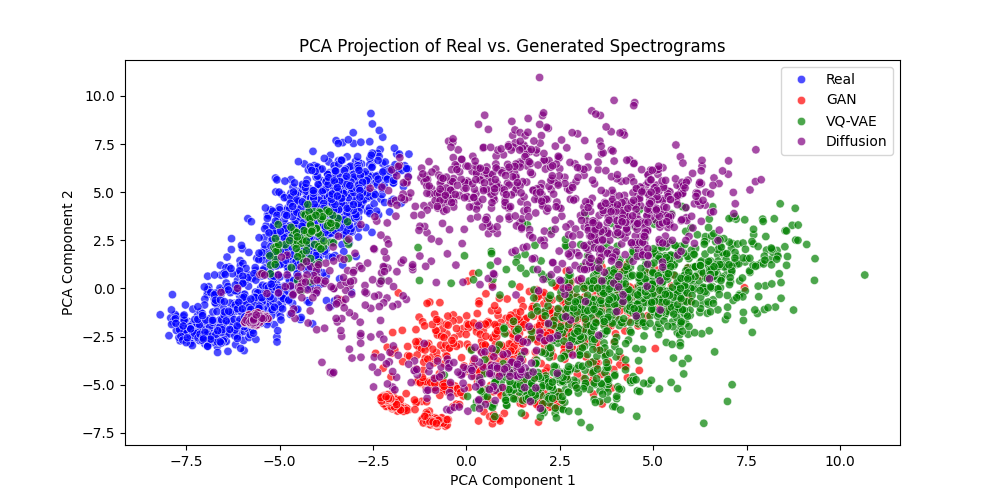
\includegraphics[width=\textwidth]{figures/PCA (1).png}
\centering
\caption{ \gls{pca} scores for the \gls{gan}, \gls{ddpm} and \gls{vq-vae}}
\centering
\end{figure}
The \gls{pca} projection in Figure 3.3 indicate that real and generated spectrograms form separate yet overlapping clusters, suggesting that generative models do not simply reproduce existing samples but introduce new variations. The spread of generated samples in the \gls{pca} projection indicates that the models create additional variations, potentially improving classifier generalization. The \gls{pca} analysis provides an independent validation of data distribution differences, confirming that generative models add meaningful diversity.
However, the \gls{pca} projection also shows that the \gls{gan} model's generated samples are more clustered and less spread out than the other two models, indicating that the \gls{gan} model may not be as effective at generating diverse samples as the \gls{ddpm} and \gls{vq-vae} models. The \gls{ddpm} model's generated samples are more spread out than the \gls{vq-vae} model's, suggesting that the \gls{ddpm} model may be more effective at generating diverse samples than the \gls{vq-vae} model.


\begin{figure}[t]
    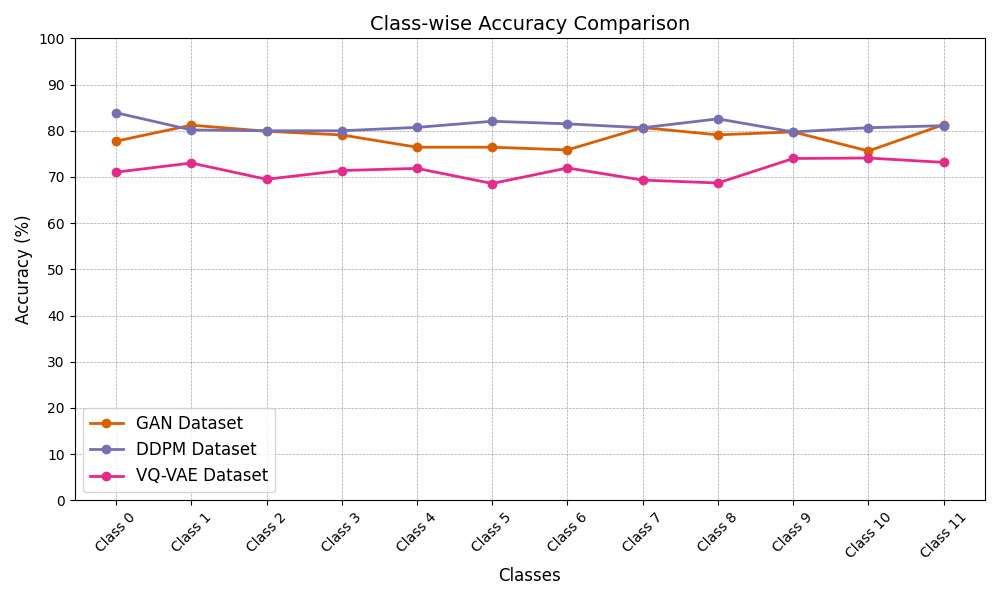
\includegraphics[width=8.5cm]{figures/Figure_20 (1).png}
    \centering
    \caption{Class-wise classification accuracy for \gls{gan}, \gls{ddpm} and \gls{vq-vae} generated data}
    \centering
    \end{figure}
    
    Figure 3.4 illustrates the change in the classification accuracy of the \gls{cnn} model for the spectrogram images generated by the three generative models for the twelve different data classes. Meanwhile, the spectrogram images generated by the \gls{ddpm} generally outperformed the images generated by other models. Even though we used a \gls{cnn} model specifically trained to distinguish fine-grained features ignoring the noise, the high noise and blurry features in the \gls{vq-vae} model seem to have affected the accuracy of the \gls{cnn} model than the other two models. 
    
    
    \begin{table}[h!]
        \centering
        \begin{tabular}{c c c c}
            \hline
            Cases & Model & Average Accuracy & \gls{fid} Score \\
            \hline
            1 & \gls{ddpm} & 81.9\% & 0.504\\
            \hline
            2 & \gls{gan} & 78.5\% & 1.944\\
            \hline
            3 & \gls{vq-vae} & 71.3\%  & 1.580\\
            \hline
        \end{tabular}
        \caption{Average accuracy for \gls{gan}, \gls{ddpm}, and Original data}
        \label{tab:average_accuracy}
    \end{table}
    
    Table 1 depicts the average classification accuracy and the \gls{fid} scores of the spectrogram images, for the three different models and the original data.
    Although the average accuracy is not far apart for the three generative models, due to the lack of diversity of the generated data by the \gls{gan}, and the noisy images by \gls{vq-vae} we can conclude that the \gls{ddpm} performs better than the \gls{gan} or \gls{vq-vae} when generating spectrogram images for a robust spectrum-sharing system.

    After calculating the classification accuracy we trained four \gls{dqn} agents using the generated data from the three models and the original data. The \gls{dqn} agents were trained for 1000 episodes. We then evaluated the trained \gls{dqn}agent based on how well the agent was able to avoid collisions using the CNN classifications of the four models in the simulated MATLAB \gls{cbrs} environment.

    
\begin{figure}[htbp]
    \centering
    \begin{subfigure}[b]{0.45\textwidth}
        \centering
        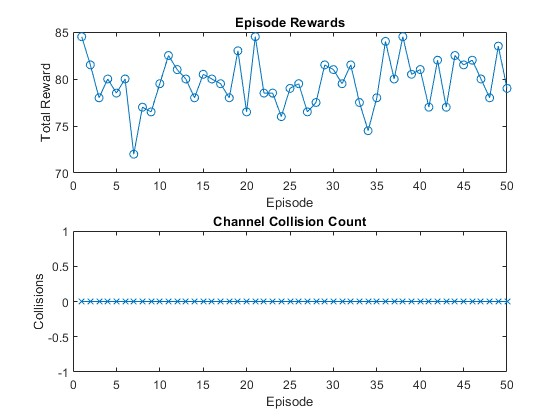
\includegraphics[width=\linewidth]{figures/collision_count_ddpm.jpg}
        \caption{DDPM}
    \end{subfigure}
    \hfill
    \begin{subfigure}[b]{0.45\textwidth}
        \centering
        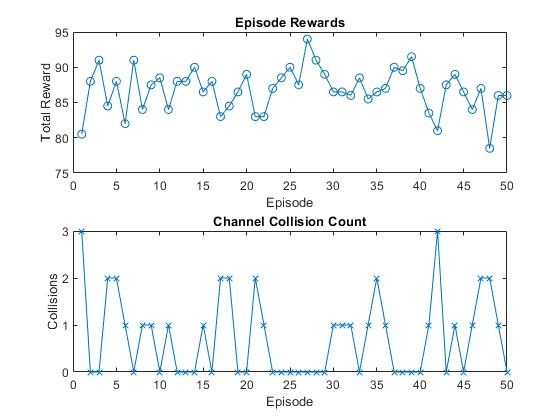
\includegraphics[width=\linewidth]{figures/collision_count_gan.jpg}
        \caption{GAN}
    \end{subfigure}

    \vspace{0.5cm} % space between rows

    \begin{subfigure}[b]{0.45\textwidth}
        \centering
        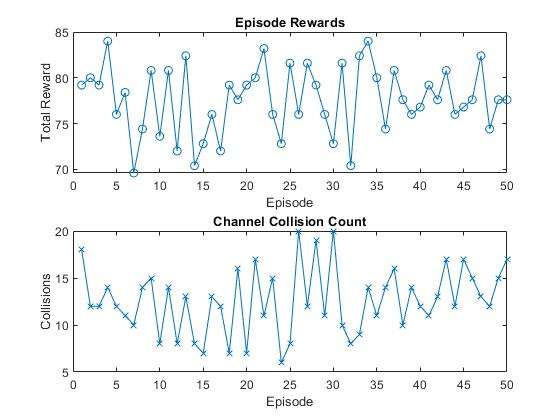
\includegraphics[width=\linewidth]{figures/collision_count_vqvae.jpg}
        \caption{VQ-VAE}
    \end{subfigure}
    \hfill
    \begin{subfigure}[b]{0.45\textwidth}
        \centering
        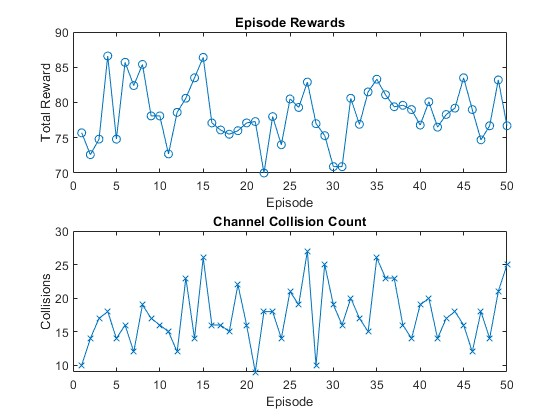
\includegraphics[width=\linewidth]{figures/collision_count_original.jpg}
        \caption{Original dataset}
    \end{subfigure}

    \caption{Performance of DQN agents trained with the four different datasets}
\end{figure}

\begin{table}[ht]
    \centering
    \caption{Comparison of Generative Models in Terms of Mean Reward and Collision Rate}
    \begin{tabular}{|l|c|c|}
    \hline
    \textbf{Model} & \textbf{Mean Reward} & \textbf{Mean Collisions per Episode} \\
    \hline
    DDPM     & 79.65   & 0.00    \\
    GAN      & 86.78   & 0.74    \\
    VQ-VAE   & 77.62   & 12.60   \\
    Original & 78.40   & 17.44   \\
    \hline
    \end{tabular}
    \label{tab:reward_collision_comparison}
\end{table}
   
    Figure 3.5 and Table 3.1 depicts the performance of DQN agents trained with datasets generated using DDPM, GAN, VQ-VAE, and the original dataset. The DDPM-trained agent exhibits highly stable behavior, achieving a consistently high reward across episodes with zero collisions—indicating excellent generalization and safe spectrum selection. The GAN-based agent demonstrates the highest average reward among all models; however, it incurs occasional collisions, suggesting a trade-off between performance and safety. In contrast, the VQ-VAE-trained agent shows high variability in both rewards and collisions, implying that its synthetic data may introduce noise or uncertainty, leading to less reliable policy learning. Lastly, the agent trained on the original dataset performs moderately well in terms of reward but experiences the highest average collision rate, underscoring the benefit of augmenting training with high-quality synthetic data like that from DDPM. These results collectively highlight that generative models, especially DDPM, can significantly enhance the safety and performance of DQN agents in dynamic spectrum access scenarios.



%%%%%%%%%%%%%%%%
% Chapter 4
%%%%%%%%%%%%%%%%

\chapter{Discussion}
\label{chap:discussion}

In this paper, we presented a deep learning-based system for interference classification in the \gls{cbrs} spectrum, leveraging synthetic data generated by three distinct generative models: \gls{gan}s,\gls{ddpm}s, and \gls{vq-vae}s. A \gls{cnn} was trained using the datasets produced by each generative model, and the classification accuracies were compared. Then that pre-trained \gls{cnn} was used to detect Incumbent users in a simulated CBRS environment with a \gls{drl} agent for channel allocation. The performance of the \gls{drl} agent and the \gls{cnn} was measured Additionally, the \gls{fid} was used to evaluate the quality and diversity of the images generated by the models.  

The experimental results show that the images generated by \gls{ddpm}, \gls{gan}, and \gls{vq-vae} achieved classification accuracies of 81.9\%, 78.5\%, and 71.3\%, respectively. Among the three models, \gls{ddpm} achieved the lowest \gls{fid} score, indicating that it produced images with the highest diversity while maintaining fidelity. These findings suggest that \gls{ddpm}-generated datasets when combined with \gls{cnn}-based classification, provide the most effective approach for interference classification in the \gls{cbrs} spectrum. The combination of superior classification accuracy and low \gls{fid} score underscores the advantage of \gls{ddpm} in this application.  

Furthermore, the performance of \gls{dqn} agents trained using each generative model was analyzed in terms of reward and safety in a simulated CBRS environment. The \gls{ddpm}-trained agent showed the best safety profile, maintaining a mean reward of 79.65 with zero collisions per episode, demonstrating strong generalization and conservative channel selection. The \gls{gan}-trained agent achieved the highest mean reward of 86.78, though it incurred an average of 0.74 collisions per episode, reflecting a more aggressive but risk-prone strategy. In contrast, the \gls{vq-vae}-trained agent had a lower mean reward of 77.62 and suffered from 12.6 collisions per episode, while the agent trained on the original dataset yielded a reward of 78.4 with 17.44 collisions per episode. These results highlight the effectiveness of \gls{ddpm} in producing not only high-quality training data but also enabling safe and efficient decision-making by reinforcement learning agents in dynamic spectrum-sharing settings.

While the proposed system is tailored for collision detection and spectrum management within \gls{cbrs}, its architecture and methodology are inherently adaptable to other dynamic spectrum-sharing frameworks. The use of generative models such as \gls{ddpm}s, \gls{gan}s, and \gls{vq-vae}s for creating synthetic collision scenarios and training robust classifiers is not limited to \gls{cbrs} but can be extended to any system that requires dynamic interference management and real-time decision-making.  

For instance, \gls{tvws}\cite{13}, which allow unlicensed devices to operate in unused portions of the broadcast television spectrum, face challenges similar to \gls{cbrs} in managing interference between primary and secondary users. The synthetic data generation techniques presented in this work can aid in training deep learning classifiers for detecting spectrum misuse or interference in such systems.  

Additionally, this approach is well-suited for 5G and 6G networks, where ultra-dense deployments and diverse spectrum use cases demand advanced interference detection and management capabilities. In these environments, generative models can simulate interference scenarios across various network slices, enabling operators to develop more resilient \gls{dsa} systems.  

An important future research direction is addressing the challenge of distinguishing between \gls{pal} and \gls{gaa} users, particularly in scenarios where their spectral behavior appears identical. One promising approach could involve incorporating network-level information, such as decoding the System Information Block (SIB1)  message to retrieve the \gls{mnc} of colliding networks. This would allow for identifying the specific networks involved in suspected \gls{pal} and \gls{gaa} collisions. Integrating tools such as Keysight Nemo with the proposed deep learning framework could create a hybrid system where spectral analysis detects potential collisions and network monitoring tools provide additional validation and identification. This complementary methodology offers a pathway for further enhancing spectrum management and interference classification strategies. 



%%%%%%%%%%%%%%%%
% Chapter 5
%%%%%%%%%%%%%%%%

\chapter{Conclusion}
\label{chap:conclusion}

Lorem ipsum dolor sit amet, consectetur adipiscing elit, sed do eiusmod tempor incididunt ut labore et dolore magna aliqua. Ut enim ad minim veniam, quis nostrud exercitation ullamco laboris nisi ut aliquip ex ea commodo consequat \textcite{ref1}. Duis aute irure dolor in reprehenderit in voluptate velit esse cillum dolore eu fugiat nulla pariatur \textcite{ref2}. Excepteur sint occaecat cupidatat non proident, sunt in culpa qui officia deserunt mollit anim id est laborum \textcite{ref3}.

%%%%%%%%%%%%%%%%
% References
%%%%%%%%%%%%%%%%
% \nocites


\setlength\bibitemsep{\baselineskip}  %manually set separataion betwen items in bibliography to double space



\printbibliography[title={References}]




\addcontentsline{toc}{chapter}{References}  %add References section to Table of Contents


% To fix incorrect incorrect page numbering in ToC, add cleardoublepage and phantomsection
% https://tex.stackexchange.com/questions/23499/incorrect-bookmarks-and-page-number-in-table-of-contents




\cleardoublepage
\phantomsection
\addcontentsline{toc}{chapter}{국문초록}  %add References section to Table of Contents
\clearpage
\begin{flushleft}
    \Large{
        \textbf{국 문 초 록}\\
    }
\vspace{\baselineskip}
\end{flushleft}

\begin{centering}
    \LARGE{
        \textbf{딥러닝 및 생성 인공지능 모델을 활용한 동적 스펙트럼 공유} \\
    }
\vspace{\baselineskip}
\end{centering}


\begin{flushright}
    Gamage Amanda Sheron \\
    전기전자공학부 \\
    연세대학교 일반대학원
\end{flushright}

동적 스펙트럼 공유는 무선 통신 자원의 효율적인 활용을 위한 핵심 요소이며, 특히 Citizens Broadband Radio Service (CBRS) 대역에서 중요한 역할을 한다. 
본 학위논문에서는 생성 모델링, 지도 학습 기반 분류, 그리고 Deep Reinforcement Learning(DRL)을 통합한 지능형 스펙트럼 액세스를 위한 새로운 종단 간 AI 기반 프레임워크를 
제안한다. 제안하는 시스템은 전통적인 Spectrum Access System (SAS)을 대체할 수 있는 학습 기반 대안으로, 실시간 스펙트럼 점유 탐지 및 자율 채널 선택을 
수행할 수 있도록 설계한다.

학습을 위한 레이블링 데이터의 부족 문제를 해결하기 위해, 본 논문에서는 세 가지 종류의 생성 AI 모델—Generative Adversarial Network (GAN), Vector Quantize Auto Encoder (VQ-VAE),
Denoising Diffusion Probabilistic Model (DDPM)—을 활용하여 간섭 및 충돌 사례를 포함한 다양한 CBRS 시나리오를 나타내는 고품질 스펙트로그램 이미지를 생성한다. 이렇게 생성된 
합성 스펙트로그램은 충돌 이벤트의 이진 분류를 위한 Convolution Neural Network (CNN) 학습에 사용한다. 실험 결과에 따르면, 시각적 품질과 분류 정확도 모두에서 DDPM이 가장 우수한 
성능을 보이며, GAN 및 VQ-VAE를 크게 상회하는 결과를 보인다.

MATLAB 기반의 CBRS 시뮬레이션 환경을 구축하고, 이 환경에서 Deep Q- Network (DQN)을 사용하여 학습된 DRL 에이전트가 스펙트럼 환경과 상호작용한다. 에이전트는 CNN으로부터 채널 점유 예측을 
받아 Incumbent 사용자 및 Priority Access License (PAL) 사용자와의 충돌을 피하면서 General Authorized Access (GAA) 채널에서의 처리량을 극대화하도록 학습한다. 정량적 결과에 따르면, 
DDPM으로 생성한 데이터를 활용해 학습한 DQN 에이전트는 에피소드당 평균 보상 79.65와 충돌 0건이라는 안전하고 효과적인 채널 선택 성능을 보인다. 반면, GAN 기반 에이전트는 더 높은 평균 
보상(86.78)을 달성하였으나 에피소드당 평균 충돌이 0.74건 발생하였고, VQ-VAE 및 실제 데이터 기반 에이전트는 각각 12.6건 및 17.44건의 높은 충돌률을 보이며 보상 또한 낮거나 유사한 수준에 
머무른다. 이러한 결과는 생성 모델의 품질이 스펙트럼 액세스에서의 성능과 운영 안전성을 모두 보장하는 데 있어 매우 중요함을 시사한다.

본 논문은 생성 AI, 심층 분류, 그리고 DRL의 통합이 CBRS 대역에서의 스펙트럼 공유 문제에 대해 확장 가능하고 지능적인 해결책을 제공함을 결론짓는다. 제안하는 모듈형 아키텍처, 고성능 학습 모델, 
그리고 시뮬레이션 결과는 향후 멀티채널 확장, 실시간 배포, 비지도 학습 기반 스펙트럼 관리 기법 등의 연구 확장을 위한 기반을 마련한다.

\blfootnote{핵심어: Citizens Broadband Radio Service (CBRS), Generative Adversarial Network (GAN), Vector Quantize Auto Encoder (VQ-VAE), Denoising Diffusion Probabilistic Model (DDPM), 
Deep Q- Network (DQN), Spectrum Access System (SAS), 동적 스펙트럼 공유, Reinforcement Learning, Convolution Neural Network (CNN)}

\end{document}
